\documentclass[10pt, a4paper]{article}
    \usepackage[utf8]{inputenc}
    %\usepackage[english, spanish]{babel}
    %\usepackage{fullpage} % changes the margin
    \usepackage{graphicx} 
    \usepackage{enumitem} 
    \usepackage{chngcntr}
    \counterwithin{figure}{section}
    \renewcommand{\thesection}{\arabic{section}} 
    \renewcommand{\thesubsection}{\thesection.\arabic{subsection}}
    \renewcommand{\baselinestretch}{1.5}

    \usepackage{amsmath}
    \usepackage{mathptmx}
    \usepackage[spanish, es-tabla]{babel}
    \usepackage{amssymb}
    \usepackage{makeidx}
    \usepackage{float}
    \pagenumbering{arabic}
    \usepackage[left=25mm, right=25mm, top=25mm, bottom=25mm]{geometry}

    \usepackage[backend=biber]{biblatex}
    \bibliography{referencias}

\begin{document}

    \begin{titlepage}
        \centering
        {\scshape\Large Universidad Central de Venezuela \par}
        {\scshape\Large Facultad de ingenier\'ia \par}
        {\scshape\Large Escuela de ingenier\'ia El\'ectrica \par}
        {\scshape\Large Departamento de Electr\'onica, Computaci\'on y Control \par}

        \vspace{6cm}
        {\Large\bfseries LABORATORIO 3 - Polarización del BJT\par}
        \vspace{5cm}

        \vfill
        %\begin{flushleft}
        %    Auxiliar docente:\par
        %    Tovar José
        %\end{flushleft}
        %\vspace{-2cm} %pendiente
        \begin{flushright}
            Estudiantes:\par
            Santana Ricardo C.I.:29571461 \par
            Fajardo Carla C.I.:27571576
            \vspace{1cm}  
        \end{flushright}
        \vfill
        {\large \today \par}
    \end{titlepage}

    \tableofcontents

    \newpage

    \section{Resumen}

    Con los circuitos necesarios previamente montados se procedió a seguir los pasos planteados en la metodología. En cuanto a las mediciones, estas se realizaron sin mayores inconvenientes ya que se tomaron previsiones al identificar todas las resistencias que se utilizarían debido a las múltiples combinaciones de resistencias que había que hacer para ciertos circuitos, con el fin de estudiar el comportamiento del transistor en sus distintas zonas de operación.

    \newpage

    \section{Introducción}

    Entre las diversas estructuras que pueden conformar los semiconductores cabe destacar la del transistor de unión bipolar, conocido por sus siglas en inglés como BJT (Bipolar Junction Transistor), ésta consta de dos uniones pn construidas de manera especial y conectadas en serie, espalda con espalda.

    El transistor consta de tres terminales, estos se denominan emisor (E), base (B) y colector (C); en base a estos el transistor puede implementarse en un circuito con configuración emisor común, base común o colector común, Se experimentará utilizando la configuración emisor común.
    
    Se presentará en el escrito las nociones básicas del BJT, de tal forma que se permita establecer el punto estático de operación que relaciona a la recta de carga y la curva característica del transistor, la cual nos facilita la implementación y diseño de circuitos electrónicos más complejos con transistores.

    \newpage

    \section{Objetivos}

    \subsection{Objetivo General}
    \begin{itemize}
        \item Análizar las características y el funcionamiento del BJT en la configuración emisor común. 
    \end{itemize}

    \subsection{Objetivos Específicos}
    \begin{itemize}
        \item Familiarizar y estudiar topologías básicas de polarización del BJT en la configuración Emisor Común.
        \item Obtener nociones acerca de la polarización del BJT.
        \item Estudiar el punto estático de operación variando el valor de las resistencias del circuito.
        \item Estudiar la recta de carga estática y su relación con las curvas características del transistor.
    \end{itemize}

    \newpage

    \section{Marco Teórico}

    El transistor BJT se describe en \cite{watson53} de la siguiente manera: 

    \subsection{Construcción del transistor}

    El transistor es un dispositivo de tres zonas o capas. Podemos tener una zona de material tipo n en medio de dos zonas de material tipo p, en este caso se denomina transistor pnp, o bien tener una zona tipo p con dos zonas tipo n a cada lado, en cuyo caso estaríamos hablando de un transistor npn.

    \begin{figure}[h!]
        \centering
        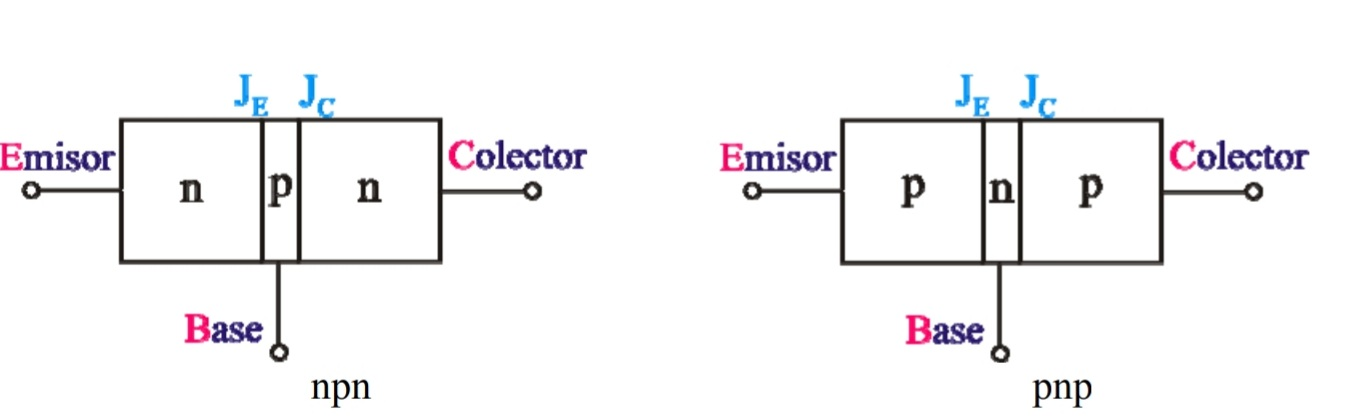
\includegraphics[height=4cm\textwidth]{construcion.jpg}
        \caption{\label{fig:1} Estructura del transistor }
    \end{figure}

    La zona central se denomina base, y las laterales emisor y colector. Cada una de las zonas consta de un terminal por donde extraer las corrientes. Estos terminales se representan por la inicial del nombre de la zona respectiva: E (emitter), B (base) y C (colector).

    \subsection{Simbolos y convenio de signos}

    \begin{figure}[h!]
        \centering
        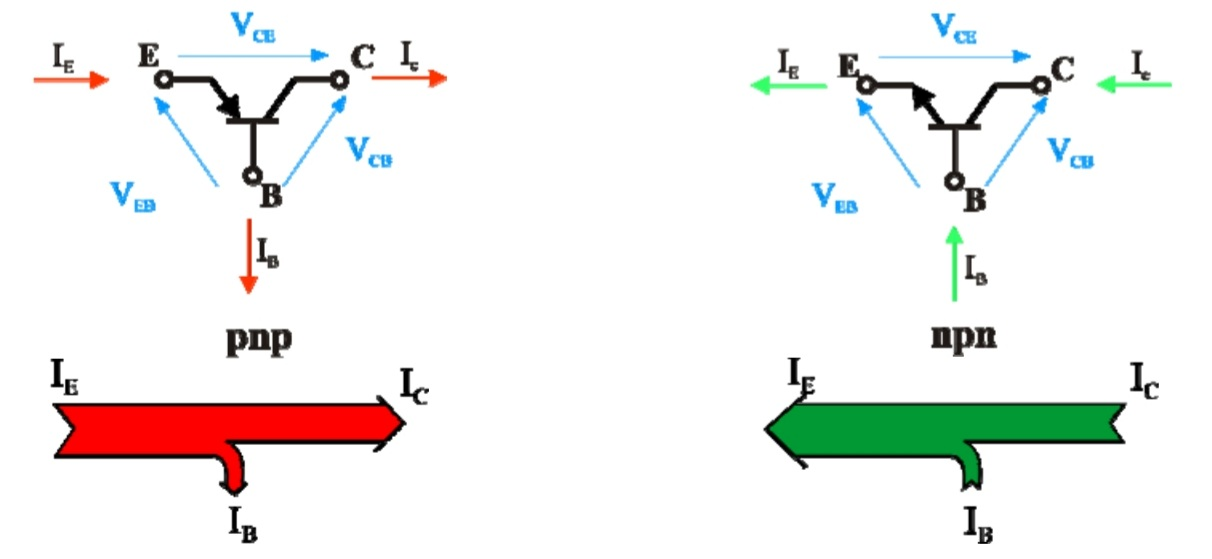
\includegraphics[height=4cm\textwidth]{simbolos.jpg}
        \caption{\label{fig:2} Estructura del transistor }
    \end{figure}

    En la figura aparecen los símbolos que se utilizan para la representación del transistor de unión bipolar. Para las corrientes se han representado los sentidos reales de circulación de las mismas.

    \subsection{zonas de funcionamiento}

    Cuando anteriormente hablábamos de la unión pn veíamos que teníamos dos posibilidades de polarización de la misma, de tal forma que el diodo tenía dos posibles estados o zonas de trabajo: en directa y en inversa. Ahora estamos ante un dispositivo que tiene dos uniones, una unión entre las zonas de emisor y base (que denominaremos a partir de ahora unión de emisor JE) y otra unión entre las zonas de base y colector (de que denominaremos unión de colector JC), cada una de las cuales puede ser polarizada en las dos formas mencionadas anteriormente. Así, desde el punto de vista global del dispositivo tenemos cuatro zonas de funcionamiento posibles en función del estado de polarización de las dos uniones.

    De esta forma, si polarizamos las dos uniones en directa, diremos que el transistor está trabajando en la zona de saturación. En el caso de que la unión de emisor la polaricemos en directa y la unión de colector en inversa, estaremos en la zona activa. Cuando las dos uniones se polarizan en inversa, se dice que el transistor está en la zona de corte. Por último, si la unión de emisor se polariza en inversa y la unión de colector en directa, el transistor se encuentra en activa inversa. De las cuatro zonas, las 3mencionadas en primer lugar son las más interesantes desde el punto de vista del funcionamiento del transistor, siendo la zona activa inversa una zona puramente teórica y sin interés práctico.

    \subsection{Curvas Características en Emisor Común}

    \subsubsection{Curvas características de entrada}

    En la siguiente figura aparecen representados los convenios de tensiones y corrientespositivas que se han tenido en cuenta para representar las distintas curvas.

    \begin{figure}[h!]
        \centering
        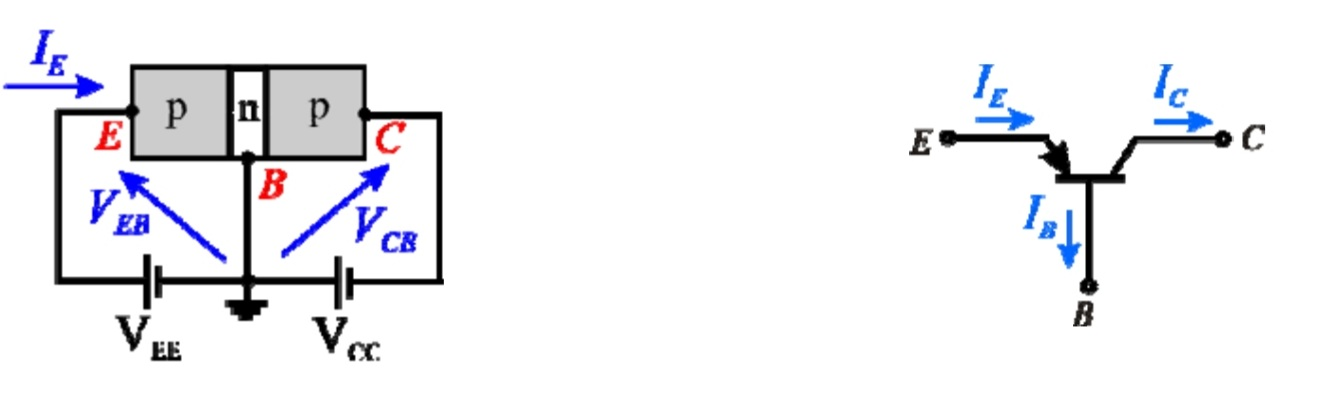
\includegraphics[height=4cm\textwidth]{entrada.jpg}
        \caption{\label{fig:3} Sentido positivo de las variable en la curva característica de entrada del BJT}
    \end{figure}

    Como se puede ver en la figura, no hay una única curva que relacione $I_B$ con $V_{BE}$, sino que hay una familia de curvas en función de $V_{CE}$.

    \begin{figure}[h!]
        \centering
        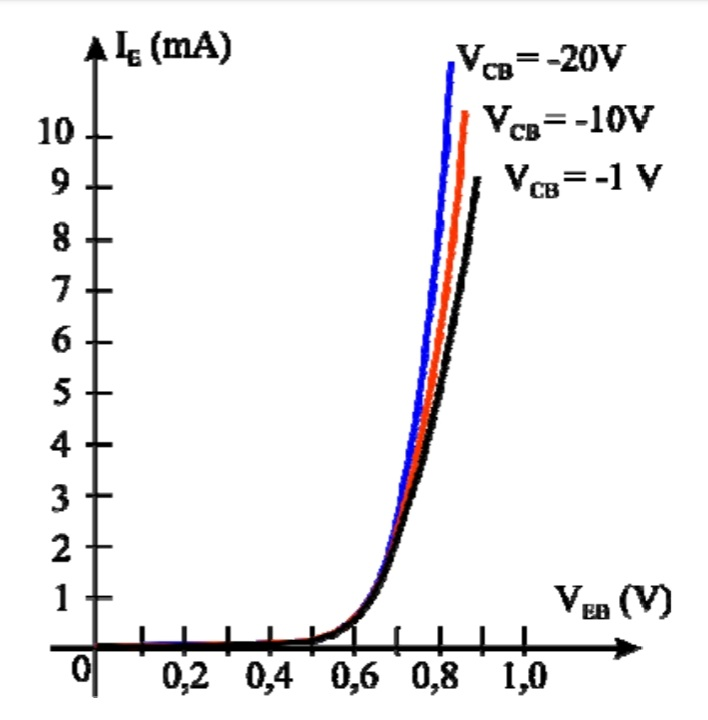
\includegraphics[height=5cm\textwidth]{graficae.jpg}
        \caption{\label{fig:4} Curvas Características de Entrada en Emsior Común para un BJT npn}
    \end{figure}

    \subsubsection{Curvas características de salida}

    \begin{figure}[h!]
        \centering
        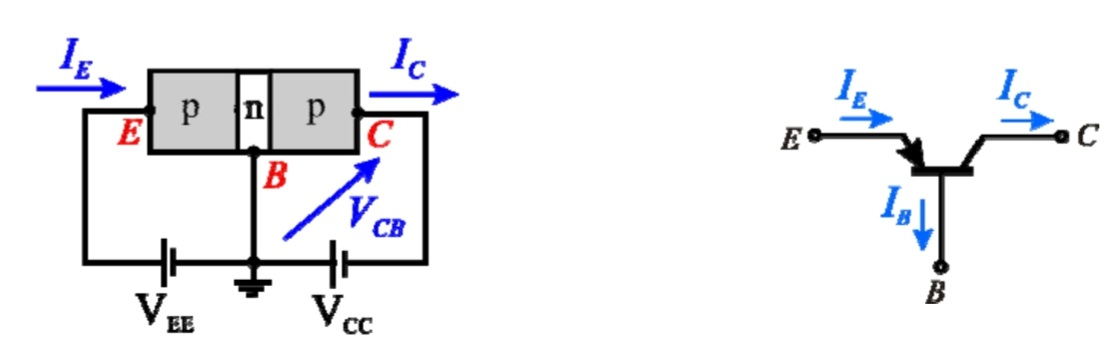
\includegraphics[height=4cm\textwidth]{salida.jpg}
        \caption{\label{fig:5} Sentido positivo de las variable en la curva característica de salida del BJT}
    \end{figure}

    En las características de salida en emisor común se representa
    
    $$I_C = f(V_{CE}, I_C)$$

    Los sentidos positivos de tensiones y corrientes son los que aparecen representados en la figura anterior

    \begin{figure}[h!]
        \centering
        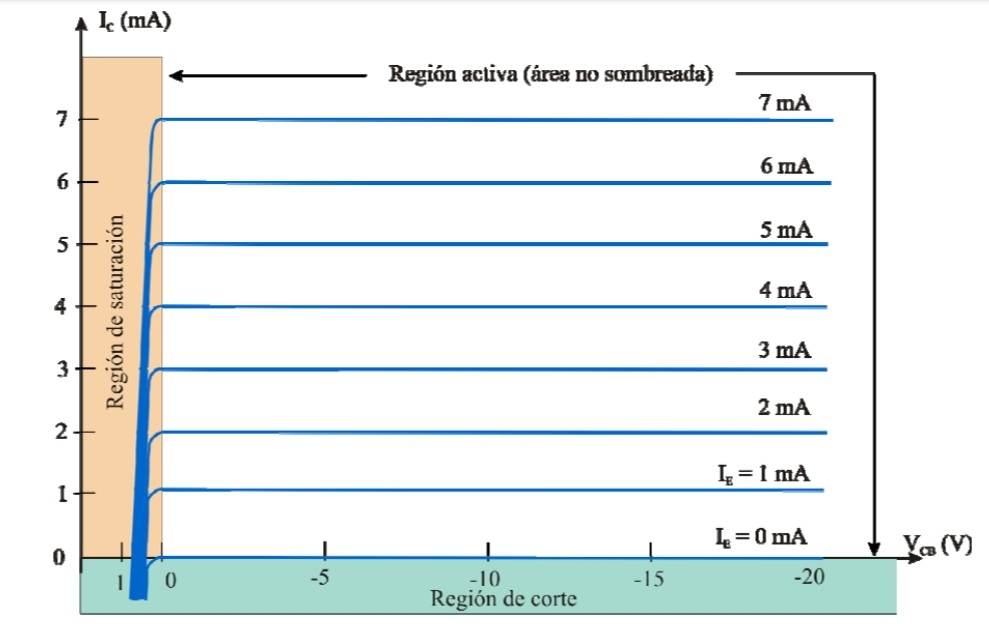
\includegraphics[height=5cm\textwidth]{graficas.jpg}
        \caption{\label{fig:6} Curvas características de salida en Emisor Común en un BJT npn}
    \end{figure}

    \newpage
    \newpage

    \section{Metodología}

    \subsection{Trabajo Previo al Laboratorio}

    \begin{enumerate}
        \item 	Determine el punto estático de operación y obtenga la tensión en cada uno de los terminales (tensión en el Colector ($V_C$), tensión en la Base (VB) y la tensión en el Emisor ($V_E$)) del BJT, para los circuitos de la Figura \ref{fig:7}, \ref{fig:8}, \ref{fig:9}, \ref{fig:10} y \ref{fig:11}. El valor de $V_{BE}$ y $\beta$, deben obtenerlo del manual del fabricante según el transistor a utilizar.
    \end{enumerate}

    \subsection{Trabajo de Laboratorio}

    \begin{enumerate}
        \item Mida la tensión en cada uno de los terminales del transistor y obtenga el punto estático de operación para el circuito de la Figura \ref{fig:7}, \ref{fig:8} y \ref{fig:9}. \label{i1}
        \item Para el circuito de la Figura \ref{fig:10} realice lo siguiente: \label{i2}
        \begin{enumerate}
            \item mida la tensión en cada uno de los terminales del transistor y obtenga el punto estático de operación. \label{pru1}
            \item mida la tensión en cada uno de los terminales del transistor y obtenga el punto estático de operación con los siguientes valores de resistencia en el circuito:
            \begin{enumerate}
                \item $RB=82k\Omega, RC=2k\Omega y RE=200\Omega.$ \label{pru2}
                \item $RB=36k\Omega, RC=2k\Omega y RE=200\Omega.$ \label{pru3}
                \item $RB=56k\Omega, RC=3k\Omega y RE=200\Omega.$ \label{pru4}
                \item $RB=56k\Omega, RC=1,3k\Omega y RE=200\Omega.$ \label{pru5}
                \item $RB=56k\Omega, RC=2k\Omega y RE=300\Omega.$ \label{pru6}
                \item $RB=56k\Omega, RC=2k\Omega y RE=130\Omega.$ \label{pru7}
            \end{enumerate}
        \end{enumerate}
        \item Para el circuito de la Figura \ref{fig:11} realice lo siguiente: \label{i3}
        \begin{enumerate}
            \item mida la tensión en cada uno de los terminales del transistor y obtenga el punto estático de operación. \label{pru8}
            \item mida la tensión en cada uno de los terminales del transistor y obtenga el punto estático de operación con los siguientes valores de resistencia en el circuito:
            \begin{enumerate}
                \item $R1=82k\Omega, R2=10k\Omega, RC=510\Omega y RE=200\Omega.$ \label{pru9}
                \item $R1=39k\Omega, R2=10k\Omega, RC=510\Omega y RE=200\Omega.$ \label{pru10}
                \item $R1=56k\Omega, R2=15k\Omega, RC=510\Omega y RE=200\Omega.$ \label{pru11}
                \item $R1=56k\Omega, R2=6,8k\Omega, RC=510\Omega y RE=200\Omega.$ \label{pru12}
                \item $R1=56k\Omega, R2=56k\Omega, RC=750\Omega y RE=200\Omega.$ \label{pru13}
                \item $R1=56k\Omega, R2=56k\Omega, RC=360\Omega y RE=200\Omega.$ \label{pru14}
            \end{enumerate}
        \end{enumerate}
        \item 	Para el circuito de la Figura \ref{fig:12}, varíe el potenciómetro de un extremo a otro, observe que ocurre con la tensión en cada uno de los terminales del transistor y el punto estático de operación. Anote en cada extremo la tensión en cada uno de los terminales del transistor y obtenga el punto estático de operación. Coloque el potenciómetro aproximadamente en la mitad de su recorrido y realice las mediciones respectivas. \label{i4}
    \end{enumerate}

    \newpage

    \begin{figure}[h!]
        \centering
        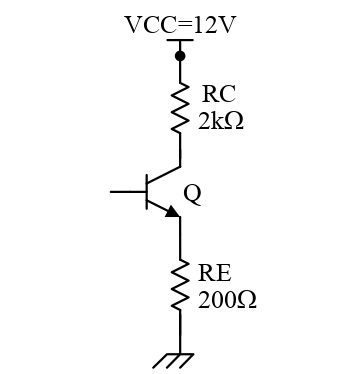
\includegraphics[height=5cm\textwidth]{circuito1.jpg}
        \caption{\label{fig:7} Circuito 1}
    \end{figure}

    \begin{figure}[h!]
        \centering
        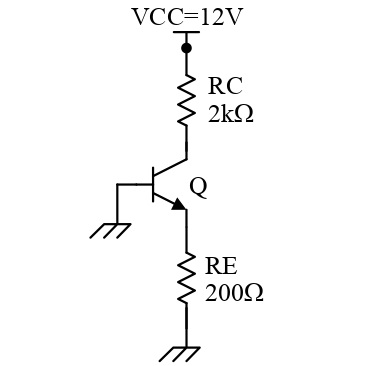
\includegraphics[height=5cm\textwidth]{circuito2.jpg}
        \caption{\label{fig:8} Circuito 2}
    \end{figure}

    \begin{figure}[h!]
        \centering
        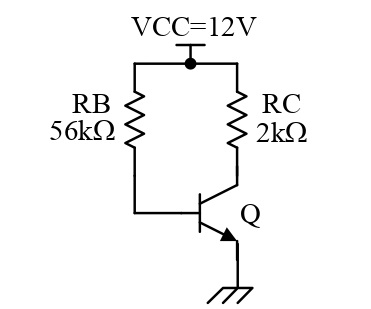
\includegraphics[height=5cm\textwidth]{circuito3.jpg}
        \caption{\label{fig:9} Circuito 3}
    \end{figure}

    \newpage

    \begin{figure}[h!]
        \centering
        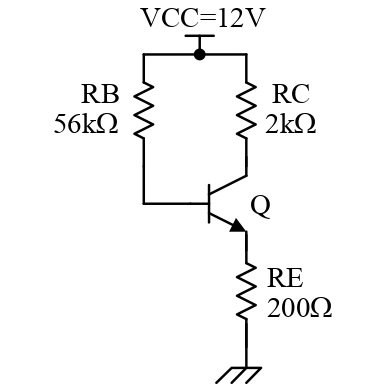
\includegraphics[height=5cm\textwidth]{circuito4.jpg}
        \caption{\label{fig:10} Circuito 4}
    \end{figure}

    \begin{figure}[h!]
        \centering
        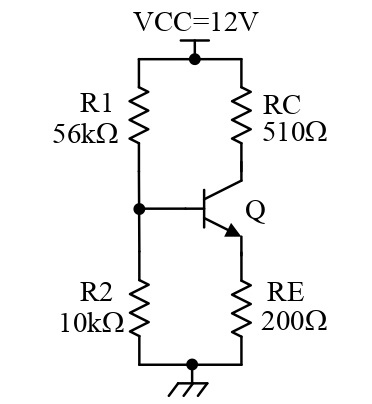
\includegraphics[height=5cm\textwidth]{circuito5.jpg}
        \caption{\label{fig:11} Circuito 5}
    \end{figure}

    \begin{figure}[h!]
        \centering
        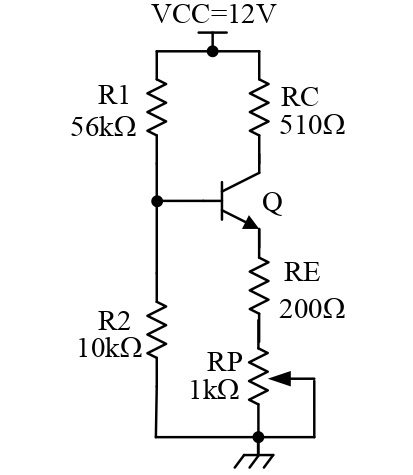
\includegraphics[height=5cm\textwidth]{circuito6.jpg}
        \caption{\label{fig:12} Circuito 6}
    \end{figure}

    \newpage

    \section{Cálculos prévios}

    Se trabajará con el transistor npn PN2222A, el cual posee las siguientes especificaciones:

    %modelo tabla
    %\begin{table}[t]
        %probar con \centering
    %    \begin{center}
    %        \begin{tabular}{| r | l |}
    %            Fruta & Cantidad \\ \hline
    %            Manzana & 4 \\
    %            Naranja & 10 \\
    %            Plátano & 3 \\ \hline
    %        \end{tabular}
    %        \caption{fruta disponible} %nombre de la tabla
    %        \label{tab:fruta} %indice de la tabla
    %    \end{center}
    %\end{table}
    
    \begin{table}[h!]
        \centering
        \caption{Características del transistor PN2222A} %nombre de la tabla
        \label{tab:especificaciones} %indice de la tabla
        \begin{tabular}{c}
            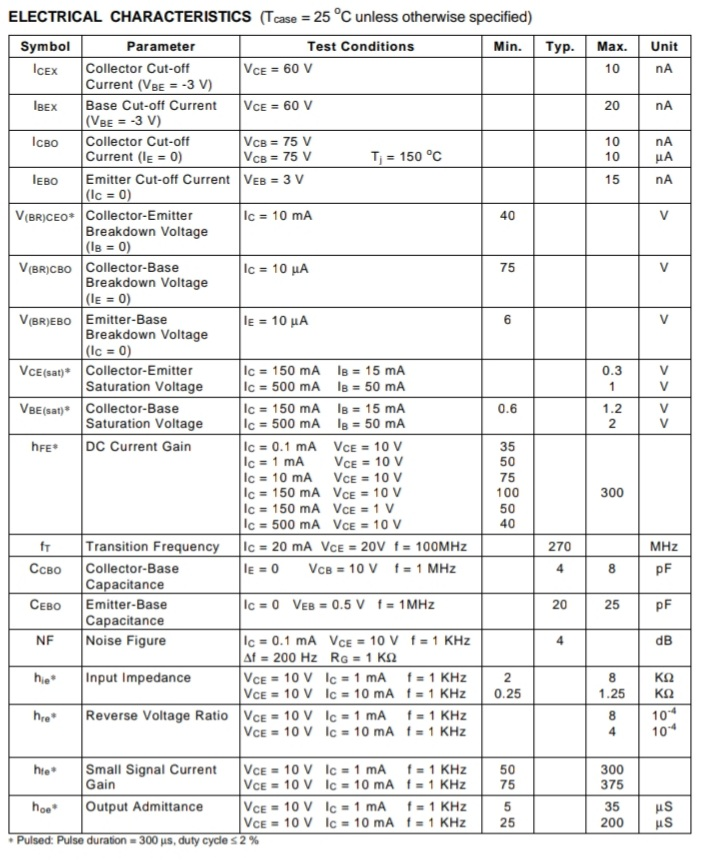
\includegraphics[height=20cm\textwidth]{pn2222a.jpg} \\
        \end{tabular}
    \end{table}

    \newpage
    
    de las cuales se deduce que:
    $$\beta = h_{FE} = 100 \; @ \; I_C = 150mA; \; V_{CE} = 10V \; (mínimo)$$
    $$V_{BEsat} = 0.6V \; @ \; I_C = 150mA; \; I_B = 15mA \; (mínimo)$$

    \subsection{Analisis del circuito de la Figura \ref{fig:7}}

    \begin{figure}[h!]
        \centering
        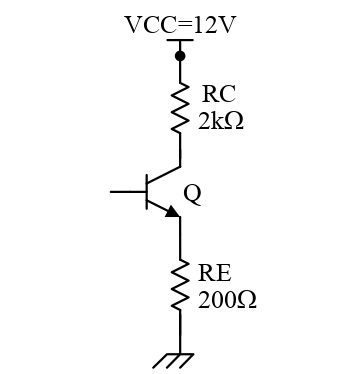
\includegraphics[height=5cm\textwidth]{circuito1.jpg} \par
        Figura \ref{fig:7}: Circuito 1 %\caption{\label{fig:7} Circuito 1}
    \end{figure}

    $V_B$ : indeterminado (circuito abierto) $\rightarrow$ asumiendo $V_B = 0V$
    Como $I_C = \beta I_B \longrightarrow I_C = 0A$, por lo tanto
    $$V_C = 12V$$
    Además $I_E = (\beta + 1)I_B \longrightarrow I_E = 0A$, por lo tanto
    $$V_E = 0V$$

    $$V_{CE} = V_C - V_E = 12V$$

    El transistor se encuentra en la zona de corte, entonces el punto de operación de la figura \ref{fig:7} es:

    \begin{equation}
        Q : (12V, 0A)
        \label{Q1}
    \end{equation}

    \subsection{Analisis del circuito de la Figura \ref{fig:8}}

    \begin{figure}[h!]
        \centering
        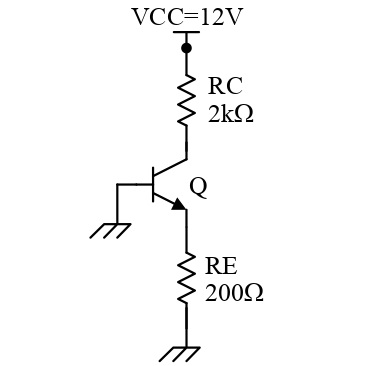
\includegraphics[height=5cm\textwidth]{circuito2.jpg} \par
        Figura \ref{fig:8}: Circuito 2 %\caption{\label{fig:5} Circuito 5}
    \end{figure}

    estimando $V_C > 0 \rightarrow V_B = 0 < V_C$, por tanto el transistor está polarizado inversamente, que indica que se encuentra en su zona de corte, entonces

    $$V_B = 0V$$

    Como $I_C = \beta I_B \longrightarrow I_C = 0A$, por lo tanto
    $$V_C = 12V$$
    Además $I_E = (\beta + 1)I_B \longrightarrow I_E = 0A$, por lo tanto
    $$V_E = 0V$$

    $$V_{CE} = V_C - V_E = 12V$$

    El transistor se encuentra en la zona de corte, entonces el punto de operación de la figura \ref{fig:8} es:

    \setcounter{equation}{1}
    \begin{equation}
        Q : (12V, 0A)
        \label{Q2}
    \end{equation}

    \subsection{Analisis del circuito de la Figura \ref{fig:9}}

    \begin{figure}[h!]
        \centering
        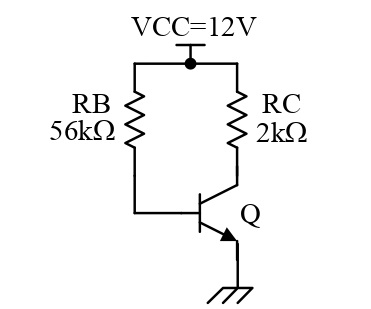
\includegraphics[height=5cm\textwidth]{circuito3.jpg} \par
        Figura \ref{fig:9}: Circuito 3 %\caption{\label{fig:5} Circuito 5}
    \end{figure}

    aplicando ley de tensiones de Kirchoff se tiene

    $$R_BI_B + V_{BE} = V_{CC}$$

    despejando $I_B$

    $$I_B = \frac{V_{CC} - V_{BE}}{R_B}$$

    sustituyendo valores

    $$I_B = \frac{12V - 0.6V}{56k\Omega} = 0.204mA$$

    aplicando ley de tensiones de Kirchoff a la malla faltante

    $$R_CI_C + V_{CE} = V_{CC}$$

    sabiendo que $I_C = \beta I_B = 20.4mA$

    $$R_C\beta I_B + V_{CE} = V_{CC}$$

    despejando $V_{CE}$

    \begin{equation}
        \label{eq1}
        V_{CE} = V_{CC} - R_C\beta I_B
    \end{equation}

    sustituyendo valores

    $$V_{CE} = 12V - 2k\Omega (100) (0.204mA) = -38.8V$$

    El transistor no se encuentra activo, entonces aplicando la lógica de los circuitos 1 y 2:

    \begin{array}{rcl}
        V_C & = & 12V \\
        V_B & = & 12V \\
        V_E & = & 0V \\
        V_{CE} & = & 12V \\
        Q & : & (12V, 0A)
    \end{array}

    por convención de signos los valores que puede llegar a tomar $V_{CE}$ quedan establecidos  en $V_{CE} > 0$

    por tanto si $V_{CE} = 0$ en \ref{eq1}:

    $$0 = 12V - R_C (100) (0.204mA)$$
    $$R_C = 588\Omega$$

    Entonces se debría cumplir que para $R_C < 588\Omega$ el transistor se encuentra saturado y circula corriente por el circuito

    \subsection{Analisis del circuito de la Figura \ref{fig:10}}

    \begin{figure}[h!]
        \centering
        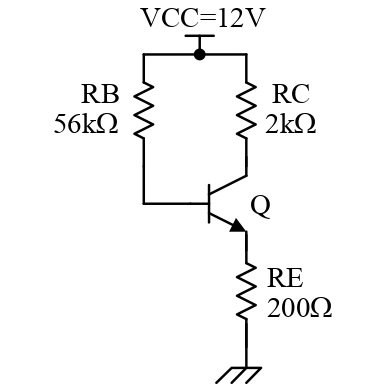
\includegraphics[height=5cm\textwidth]{circuito4.jpg} \par
        Figura \ref{fig:10}: Circuito 4 %\caption{\label{fig:5} Circuito 5}
    \end{figure}

    aplicando ley de tensiones de Kirchoff se tiene

    $$R_BI_B + V_{BE} + R_EI_E= V_{CC}$$

    sabiendo que $I_E = (\beta+1)I_B$

    $$R_BI_B + V_{BE} + R_E(\beta+1)I_B= V_{CC}$$

    despejando $I_B$

    $$I_B = \frac{V_{CC} - V_{BE}}{R_B + R_E(\beta + 1)}$$

    sustituyendo valores

    $$I_B = \frac{12V - 0.6V}{56k\Omega + 200\Omega (100 + 1)} = 0.150mA$$

    aplicando ley de tensiones de Kirchoff a la malla faltante

    $$R_CI_C + V_{CE} + R_EI_E = V_{CC}$$

    sabiendo que $I_C = \beta I_B$ y $I_E = (\beta + 1)I_B$

    $$R_C\beta I_B + V_{CE} + R_E(\beta + 1)I_B= V_{CC}$$

    despejando $V_{CE}$

    \setcounter{equation}{1}
    \begin{equation}
        \label{eq2}
        V_{CE} = V_{CC} - R_C\beta I_B - R_E(\beta + 1)I_B
    \end{equation}

    sustituyendo valores

    $$V_{CE} = 12V - 2k\Omega (100) (0.204mA) - 200 \Omega (100 + 1)(0.150mA) = -31.8V$$

    El transistor no se encuentra activo, entonces aplicando la lógica de los circuitos 1 y 2:

    \begin{array}{rcl}
        V_C & = & 12V \\
        V_B & = & 12V \\
        V_E & = & 0V \\
        V_{CE} & = & 12V \\
        Q & : & (12V, 0A)
    \end{array}

    por convención de signos los valores que puede llegar a tomar $V_{CE}$ quedan establecidos  en $V_{CE} > 0$

    por tanto si $V_{CE} = 0$ en (2):

    $$0 = 12V - R_C (100) (0.204mA) - R_E (100 + 1)(0.150mA)$$
    $$0.0204R_C + 0.0151R_E < 12$$

    Quedando así un sistema compatible indeterminado de una ecuación con dos incognitas, en el cual se pueden variar los valores de las resistencias de manera que el transistor se sature.

    \subsection{Analisis del circuito de la Figura \ref{fig:11}}

    \begin{figure}[h!]
        \centering
        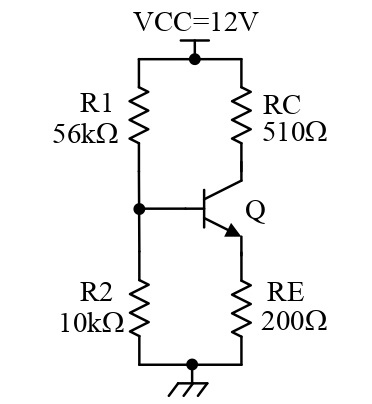
\includegraphics[height=5cm\textwidth]{circuito5.jpg} \par
        Figura \ref{fig:11}: Circuito 5 %\caption{\label{fig:5} Circuito 5}
    \end{figure}

    Calculando equivalente de thevelin entre la base del transistor y la referencia

    $$R_{Th} = R_1 // R_2 = 56k\Omega // 10k\Omega = 8.48k\Omega$$
    
    por divisor de voltaje

    $$V_{Th} = \frac{R_2}{R_1 + R_2} V_{CC} = \frac{10k\Omega}{56k\Omega + 10k\Omega} (12V) = 1.81V$$

    \begin{figure}[h!]
        \centering
        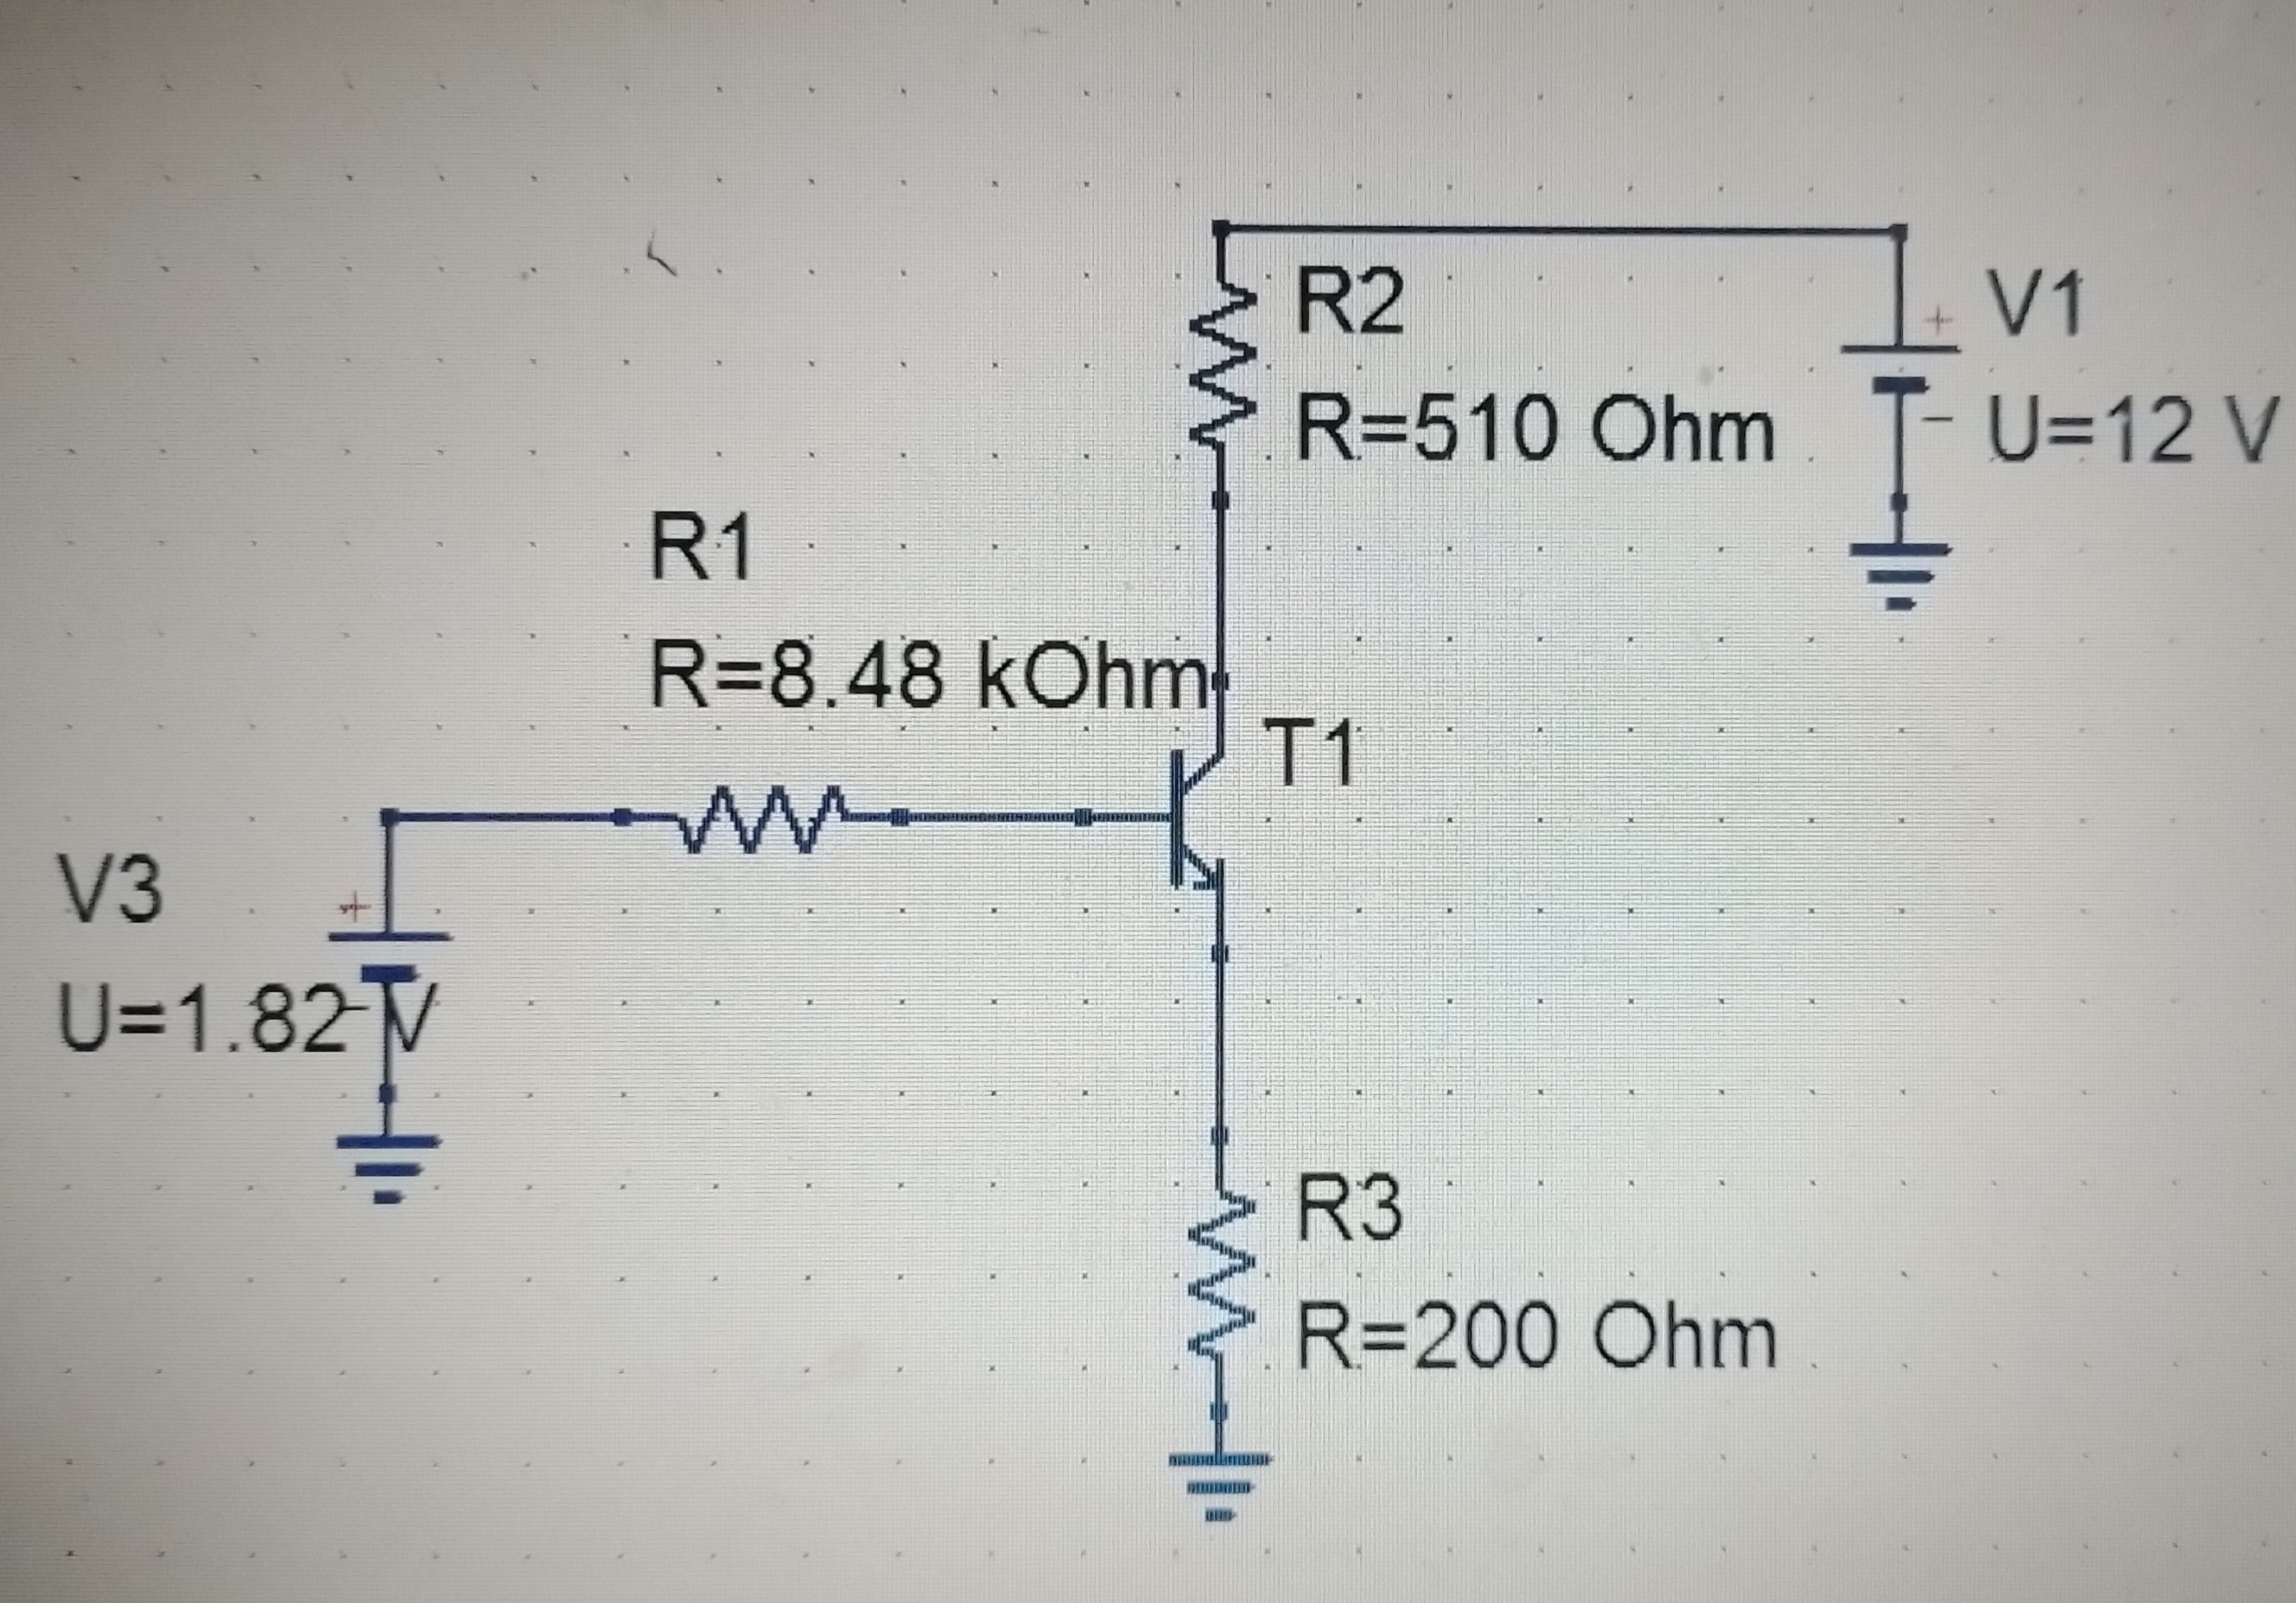
\includegraphics[height=5cm\textwidth]{thevelin5.jpg} \par
        \caption{\label{fig:13} Circuito 5 con equivalente de Thevelin}
    \end{figure}

    aplicando ley de tensiones de Kirchoff

    $$R_{Th}I_B + V_{BE} + R_EI_E = V_{Th}$$

    si $I_E = (\beta + 1)I_B$, entonces

    $$R_{Th}I_B + V_{BE} + R_E(\beta + 1)I_B = V_{Th}$$

    $$I_B = {V_{Th} - V{BE} \over R_{Th} + R_E(\beta + 1)}$$

    Sustituyendo valores

    $$I_B = {1.82V - 0.6V \over 8,48k\Omega + 200\Omega(100 + 1)} = 0.043mA$$

    sabiendo que $I_C = \beta I_B$

    $$I_C = 100(0.043mA) = 4.3mA$$

    por otra parte

    $$I_E = (\beta + 1)I_B = (100 + 1)0.043mA = 4.343mA$$

    aplicando ley de tensiones de Kirchoff a la otra malla

    $$R_{C}I_C + V_{CE} + R_EI_E = V_{CC}$$

    $$V_{CE} = V_{CC} - R_{C}I_C - R_EI_E$$

    sustituyendo

    $$V_{CE} = 12V - 510\Omega (4.3mA) - 200\Omega (4.343mA) = 8.94V$$

    por ley de ohm

    $$V_E = R_EI_E = 200\Omega (4.343mA) = 0.87V$$

    además

    $$V_B = V_{BE} + V_E = 0.6V + 0.87V = 1.47V$$

    $$V_C = V_{CE} + V_E = 8.94V + 0.87V = 9.81V$$

    punto de operacion

    \setcounter{equation}{1}
    \begin{equation}
        Q = (8.94V, 4.30mA)
        \label{Q5}
    \end{equation}

    El transistor se encuentra activo

    \subsection{Analisis del circuito de la Figura \ref{fig:12}}

    \begin{figure}[h!]
        \centering
        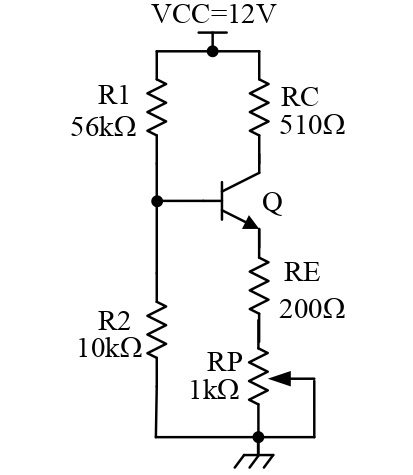
\includegraphics[height=5cm\textwidth]{circuito6.jpg} \par
        Figura \ref{fig:12}: Circuito 6 %\caption{\label{fig:5} Circuito 5}
    \end{figure}

    Se aplicará una lógica semejante al circuito anterior, donde:

    $$R_{Ecircuito5} = R_{Ecircuito6} + R_P$$

    Calculando equivalente de thevelin entre la base del transistor y la referencia

    $$R_{Th} = R_1 // R_2 = 56k\Omega // 10k\Omega = 8.48k\Omega$$
    
    por divisor de voltaje

    $$V_{Th} = \frac{R_2}{R_1 + R_2} V_{CC} = \frac{10k\Omega}{56k\Omega + 10k\Omega} (12V) = 1.81V$$

    \begin{figure}[h!]
        \centering
        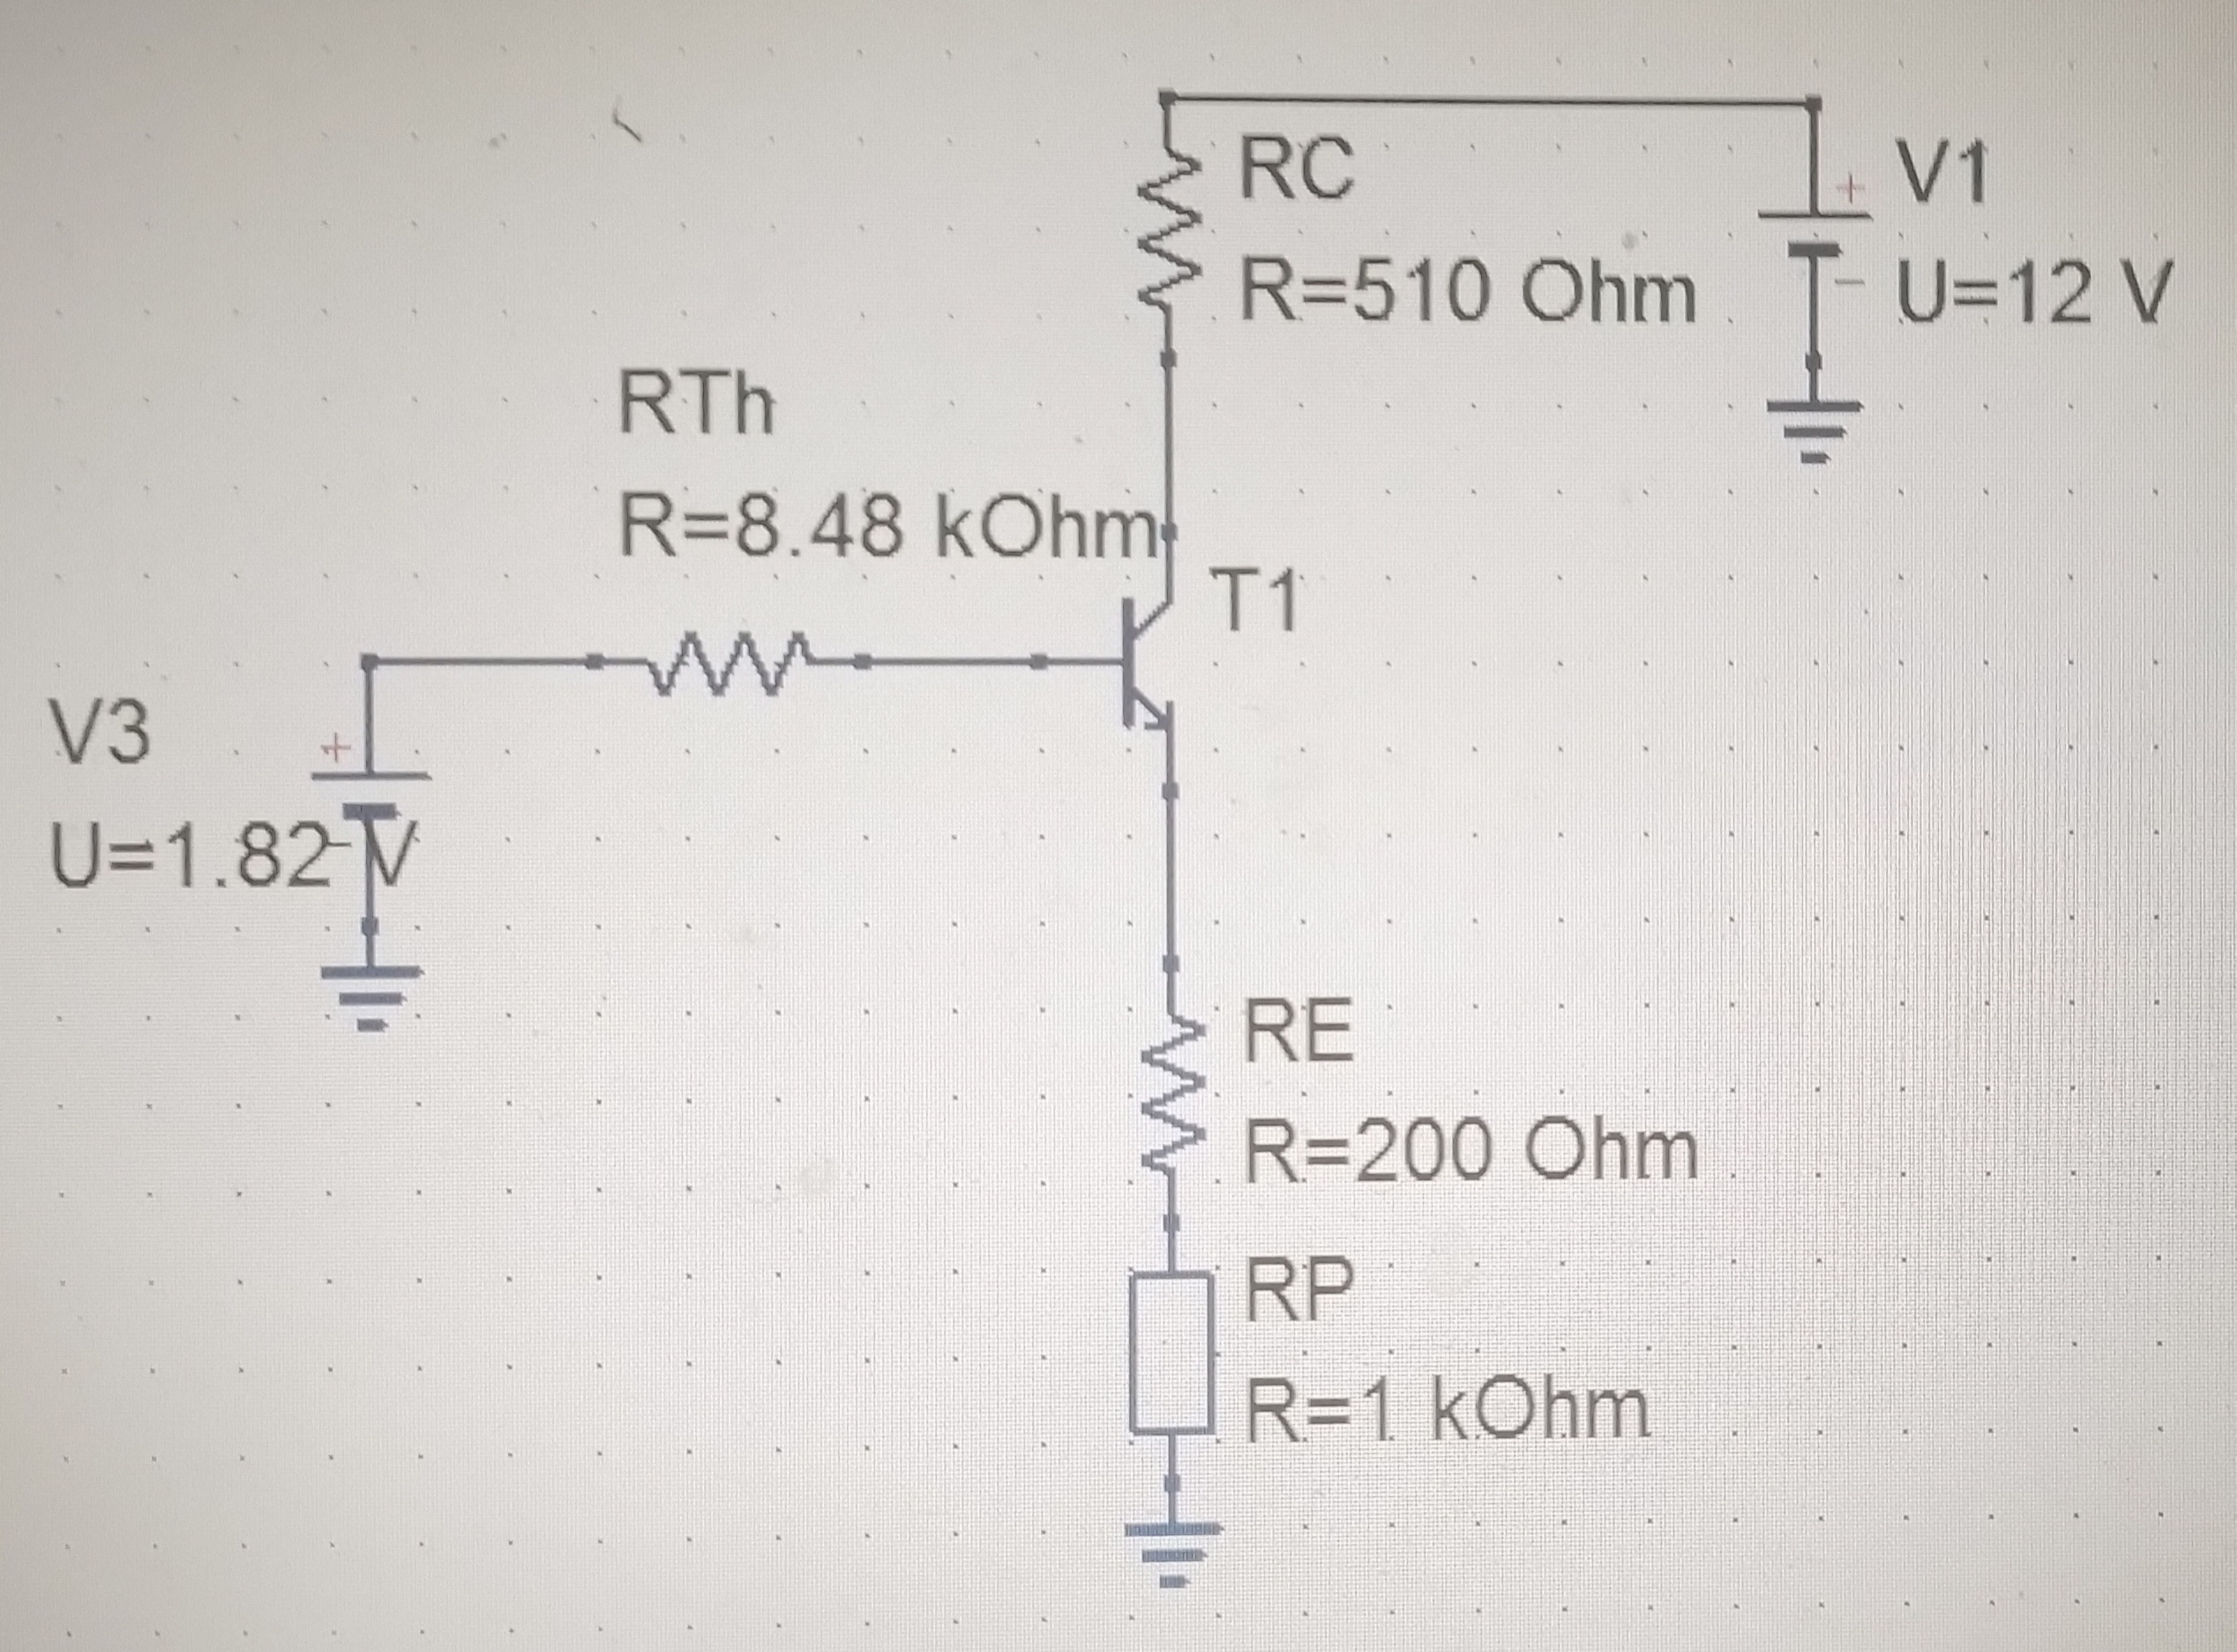
\includegraphics[height=5cm\textwidth]{thevelin6.jpg} \par
        \caption{\label{fig:14} Circuito 6 con equivalente de Thevelin}
    \end{figure}

    aplicando ley de tensiones de Kirchoff

    $$R_{Th}I_B + V_{BE} + (R_E + R_P)I_E = V_{Th}$$

    si $I_E = (\beta + 1)I_B$, entonces

    $$R_{Th}I_B + V_{BE} + (R_E + R_P)(\beta + 1)I_B = V_{Th}$$

    $$I_B = {V_{Th} - V{BE} \over R_{Th} + (R_E + R_P)(\beta + 1)}$$

    Sustituyendo valores

    $$I_B = {1.82V - 0.6V \over 8,48k\Omega + (200\Omega + R_P)(100 + 1)} = {1.22 \over 28680 +101R_P} A$$

    sabiendo que $I_C = \beta I_B$

    $$I_C = 100({1.22 \over 28680 +101R_P})A = {122 \over 28680 +101R_P}A$$

    por otra parte

    $$I_E = (\beta + 1)I_B = (100 + 1)({1.22 \over 28680 +101R_P})A = {123.22 \over 28680 +101R_P}A$$

    aplicando ley de tensiones de Kirchoff a la otra malla

    $$R_{C}I_C + V_{CE} + R_EI_E = V_{CC}$$

    $$V_{CE} = V_{CC} - R_{C}I_C - R_EI_E$$

    sustituyendo

    $$V_{CE} = 12V - 510\Omega ({122 \over 28680 +101R_P}A) - 200\Omega ({123.22 \over 28680 +101R_P}A)$$
    $$V_{CE} = (12 - {86864 \over 28680 +101R_P})V$$

    para caso extremo $R_P = 1k\Omega$

    $$V_{CE} = (12 - {86864 \over 28680 +101(1000)})V = 11.33V$$

    por ley de ohm

    $$V_E = R_EI_E = 200\Omega (0.950mA) = 0.19V$$

    además

    $$V_B = V_{BE} + V_E = 0.7V + 0.19V = 0.89V$$

    $$V_C = V_{CE} + V_E = 11.33V + 0.19V = 11.52V$$

    punto de operacion

    \begin{equation}
        Q = (11.33V, 0.940mA)
        \label{Q6}
    \end{equation}

    El transistor se encuentra activo, casi en zona de corte

    \subsection{Resumen Puntos de Operación estáticos}

    \begin{table}[h!]
        \centering
        \caption{Puntos de operacion estáticos teóricos}
        \label{tab:Qt}
        \begin{tabular}{|c|c|c|} \hline
            & $V_{CE}$ & I_C \\ \hline
            $Q_1$ & 12V & 0mA \\
            $Q_2$ & 12V & 0mA \\
            $Q_3$ & 12V & 0mA \\
            $Q_4$ & 12V & 0mA \\
            $Q_5$ & 8.94V & 4.30mA \\
            $Q_6$ & 11.33V & 0.940mA \\ \hline
        \end{tabular}
    \end{table}

    \newpage

    \section{Materiales e Instrumentos}

    \begin{table}[h!]
        \centering
        \caption{Equipos o instrumentos}
        \label{tab:instrumentos}
        \begin{tabular}{|c|c|c|} \hline
            Equipo                    &  Marca&    Modelo   \\ \hline
            Osciloscopio              &  UNI-T & UTD2102CEX+ \\ 
            Fuente de alimentacion DC  &  UNI-T & UTP3305-II  \\ \hline
        \end{tabular}
    \end{table}

    \begin{table}[h!]
        \centering
        \caption{Componentes y materiales}
        \label{tab:componentes}
        \begin{tabular}{|c|c|c|} \hline
            Referecia&Descripcion&    Especificaciones   \\ \hline
            RB = 82k$\Omega$   &  Resistencia&         1/2 W         \\
            RB = 36k$\Omega$   &  Resistencia&         1/4 W         \\
            RB = 56k$\Omega$   &  Resistencia&         1/8 W         \\
            RC = 2k$\Omega$    &  Resistencia&         1/4 W         \\
            RC = 3k$\Omega$    &  Resistencia&         1/4 W         \\
            RC = 1,3k$\Omega$  &  Resistencia&         1/4 W         \\
            RC = 510$\Omega$   &  Resistencia&         1/8 W         \\
            RC = 750$\Omega$   &  Resistencia&         1/4 W         \\
            RC = 360$\Omega$   &  Resistencia&         1/4 W         \\
            RE = 200$\Omega$   &  Resistencia&         1/4 W         \\
            RE = 300$\Omega$   &  Resistencia&         1/4 W         \\
            RE = 130$\Omega$   &  Resistencia&         1/4 W         \\
            R1 = 39k$\Omega$   &  Resistencia&         1/4 W         \\
            R2 = 10k$\Omega$   &  Resistencia&         1/4 W         \\
            R2 = 15k$\Omega$   &  Resistencia&         1/4 W         \\
            R2 = 6,8 k$\Omega$ &  Resistencia&         1/4 W         \\ 
            T = PN2222A    &Tansistor BJT NPN&   \\ \hline
        \end{tabular}
    \end{table}

    \newpage

    \section{Presentación de Resultados}

    \begin{table}[h!]
        \centering
        \caption{Resultados experimentales del trabajo de laboratorio \ref{i1} y punto de operación obtenido}
        \label{tab:1}
        \begin{tabular}{|c|c|c|c|c|c|c|} \hline
            \ref{i1}         & $V_B$ [V]  &$V_C$ [V] &$V_E$ [V] &$I_C$ [mA] & $V_{CE}$ [V] & operacion \\ \hline
            Circuito 1     &0 ± 0      &       12 ± 1      &       0 ± 0        &0 ± 0  &  12 ± 1 & corte \\
            Circuito 2     & 0 ± 0      &       12 ± 1      &       0 ± 0        & 0 ± 0 & 12 ± 1 & corte\\
            Circuito 3     &0,6 ± 0,04  &  0,09 ± 0,01   &    0 ± 0       &5,95 ± 1,10 &  0,09 ± 0,01  & saturado \\ \hline
        \end{tabular}
    \end{table}

    \begin{table}[h!]
        \centering
        \caption{Resultados experimentales del trabajo de laboratorio \ref{i2} y punto de operación obtenido}
        \label{tab:2}
        \begin{tabular}{|c|c|c|c|c|c|c|} \hline
            \ref{i2}   &  $V_B$ [V]       &    $V_C$ [V]      &    $V_E$ [V]      &  $I_C$[mA]&  $V_{CE}$ [V] & operación   \\ \hline
            \ref{pru1}  &  1,9 ± 0,1    &   1,5 ± 0,1&   1,2 ± 0,1   &     5,35 ± 1,08    &   0,1 ± 0,2   & saturado   \\
            \ref{pru2}&1,9 ± 0,1    &1,3 ± 0,1&   1,2 ± 0,1   & 5,35 ± 1,08&   0,1 ± 0,2   & saturado   \\
            \ref{pru3}    &1,9 ± 0,1    &   1,3 ± 0,1&   1,2 ± 0,1   &    5,35 ± 1,08&    0,1 ± 0,2  & saturado   \\
            \ref{pru4}&  1,5 ± 0,1    &   0,9 ± 0,1&   0,8 ± 0,1   &    3,70 ± 0,73      &    0,1 ± 0,2  & saturado   \\
            \ref{pru5}&   3 ± 0,2&2,2 ± 0,2     &   2,1 ± 0,2   &    7,53 ± 1,67&    0,2 ± 0,4   & saturado   \\
            \ref{pru6}&  2,4 ± 0,2&   1,7 ± 0,1&   1,6 ± 0,1   &5,15 ± 1,06    &    0,1 ± 0,2   & saturado   \\
            \ref{pru7}&  1,3 ± 0,1  &   0,7 ± 0,04 &   0,6 ± 0,04&    5,66 ± 1,08    &   0,08 ± 0,08 & saturado   \\ \hline
        \end{tabular}
    \end{table}

    \begin{table}[h!]
        \centering
        \caption{Resultados experimentales del trabajo de laboratorio \ref{i3} y punto de operación obtenido}
        \label{tab:3}
        \begin{tabular}{|c|c|c|c|c|c|c|} \hline
            \ref{i3} &  $V_B$ [V]       &    $V_C$ [V]&  $V_E$ [V]      &      $I_C$[mA]        &    $V_{CE}$ [V] & operación  \\ \hline
            \ref{pru8}   &  1,5 ± 0,1    &9 ± 1&  1,0 ± 0,1 &5,88 ± 4,50&   8 ± 1,1 & Activo \\
            \ref{pru9}    &1,2 ± 0,1    & 11 ± 1&   0,58 ± 0,04&1,96 ± 4,11& 10,42 ± 1,04 & Activo-Corte  \\
            \ref{pru10}    &2,4 ± 0,2&   7 ± 1&  1,8 ± 0,2& 9,80 ± 4,90&5,2 ± 1,2  & Activo   \\
            \ref{pru11}    &  2,2 ± 0,2&8 ± 1&  1,5 ± 0,1   &7,84 ± 4,70&   6,5 ± 1,1 & Activo \\
            \ref{pru12}    &1,2 ± 0,1&11 ± 1&    0,58 ± 0,04&    1,96 ± 4,11&10,42 ± 1,04 & Activo-corte  \\
            \ref{pru13}    & 3,2 ± 0,2&2,8 ± 0,2& 2,6 ± 0,2&12,26 ± 2,82 &0,2 ± 0,4 & Saturado \\
            \ref{pru14}    &3,8 ± 0,4&6 ± 0,44 & 3,2 ± 0,2& 16,67 ± 5,55&   2,8 ± 0,6 & Saturado\\ \hline
        \end{tabular}
    \end{table}

    \begin{table}[h!]
        \centering
        \caption{Resultados experimentales del trabajo de laboratorio \ref{i4} y punto de operación obtenido}
        \label{tab:4}
        \begin{tabular}{|c|c|c|c|c|c|c|} \hline
            RP [$\Omega$]  &$V_B$ [V]&    $V_C$ [V]    &      $V_E$ [V]      &      $I_C$[mA]        &    $V_{CE}$ [V]  & operación       \\ \hline
            1000     &   1,7 ± 0,1   &    12 ± 1     &    1,1 ± 0,1     &     0 ± 3,92       &   10,9 ± 1,1 & Corte      \\
            500   &   1,7 ± 0,1   &    11 ± 1     &    1,1 ± 0,1     &  1,96 ± 4,11     &    9,9 ± 1,1  & Activo-corte      \\
            10   &   1,6 ± 0,1   &    10 ± 1     &    1,0 ± 0,1     &  3,92 ± 4,31     &    9,0 ± 1,1   & Activo    \\ \hline
        \end{tabular}
    \end{table}

    {\bf Observación:} Para el cáculo del punto de operacion se utilizan las fórmulas \ref{Qeq1}, \ref{Qeq2}, \ref{Qeq3}, \ref{Qeq4} en los anexos.
    
    \newpage

    \begin{figure}[h!]
        \centering
        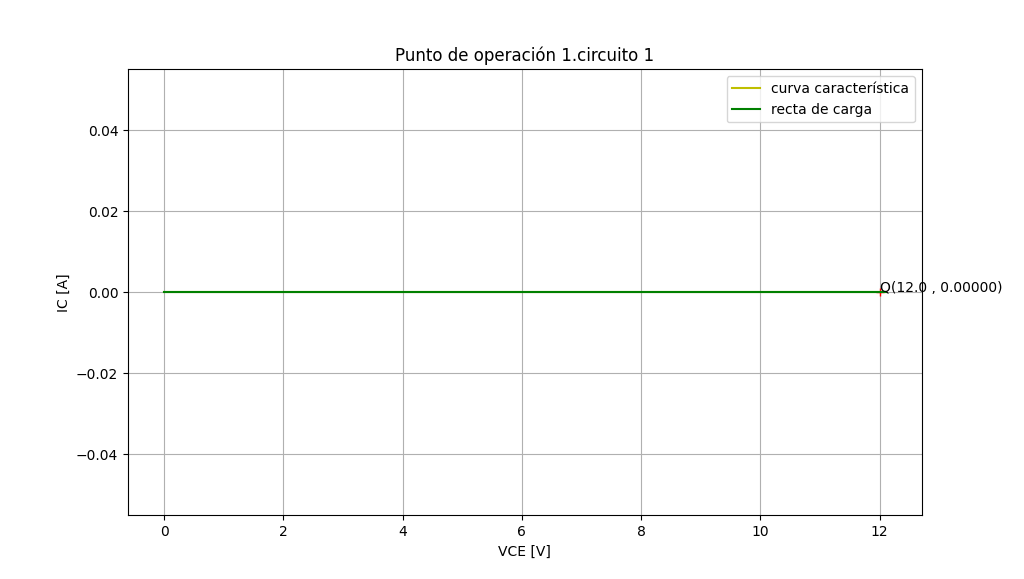
\includegraphics[height=5cm\textwidth]{1cir1.png}
        \caption{Curva Característica, recta de carga y punto de operación del circuito de la figura \ref{fig:7}}
        \label{fig:1cir1}
    \end{figure}

    \begin{figure}[h!]
        \centering
        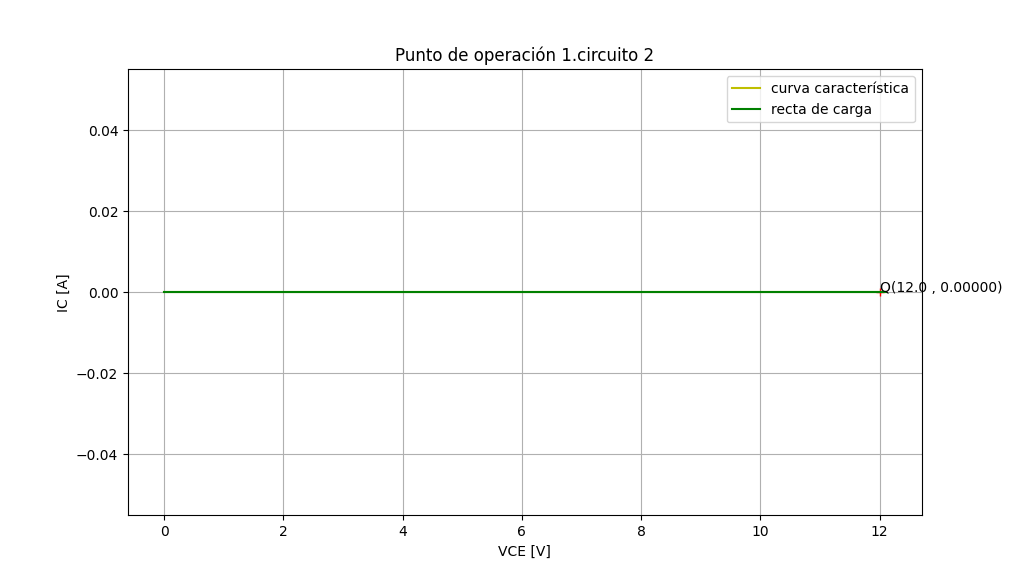
\includegraphics[height=5cm\textwidth]{1cir2.png}
        \caption{Curva Característica, recta de carga y punto de operación del circuito de la figura \ref{fig:8}}
        \label{fig:1cir2}
    \end{figure}

    \begin{figure}[h!]
        \centering
        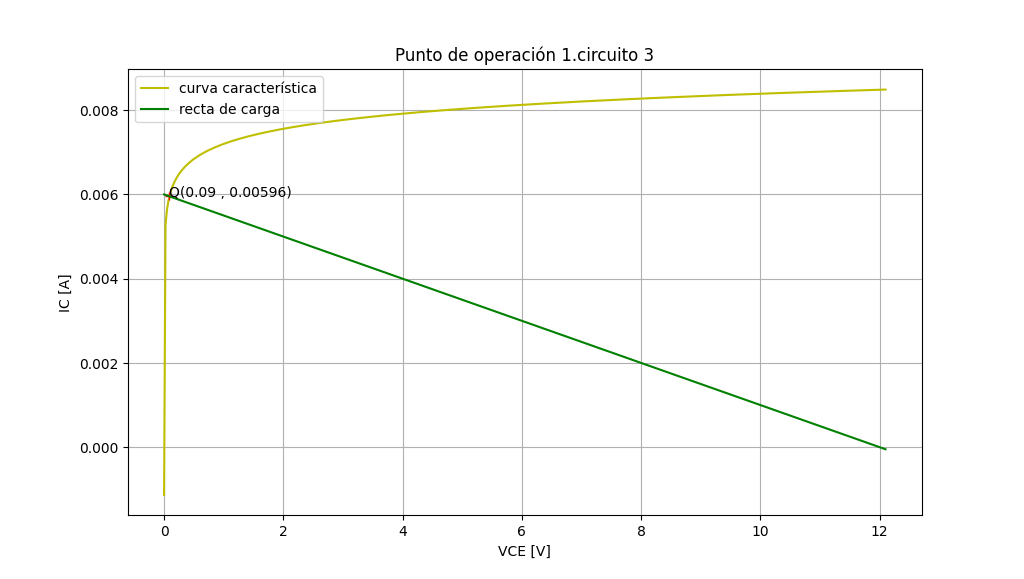
\includegraphics[height=5cm\textwidth]{1cir3.png}
        \caption{Curva Característica, recta de carga y punto de operación del circuito de la figura \ref{fig:9}}
        \label{fig:1cir3}
    \end{figure}

    \newpage

    \begin{table}[h!]
        \centering
        \caption{Valores de resistencia para la prueba de laboratorio \ref{pru1}}
        \label{tab:2a}
        \begin{tabular}{|c|c|c|} \hline
            RB & RC & RE \\ \hline
            $56k\Omega \pm 10\%$ & $2k\Omega \pm 10\%$ & $200\Omega \pm 10\%$ \\ \hline
        \end{tabular}
    \end{table}

    \begin{figure}[h!]
        \centering
        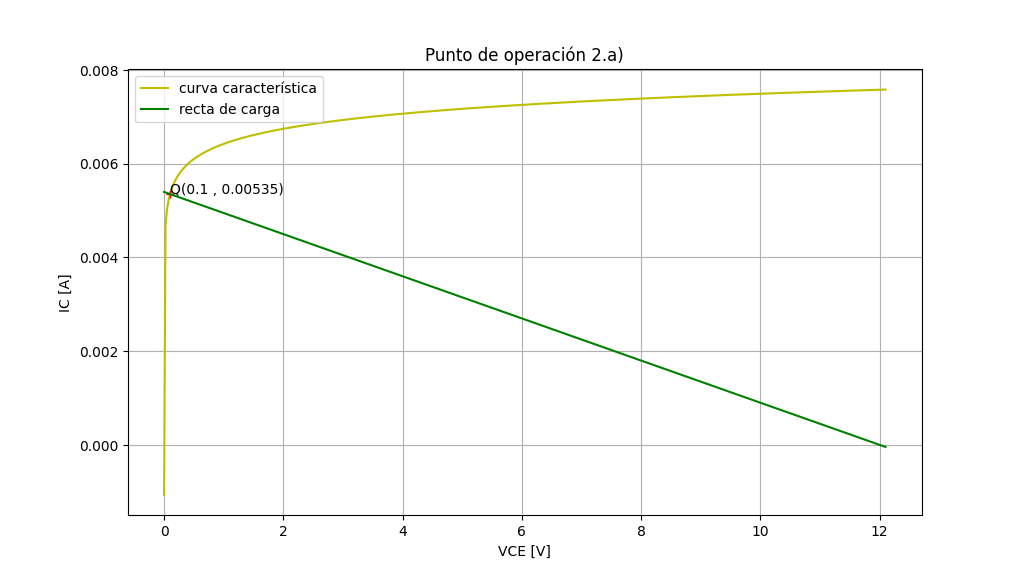
\includegraphics[height=5cm\textwidth]{2a.png}
        \caption{Curva Característica, recta de carga y punto de operación del circuito de la figura \ref{fig:10}, con valores de resistencias expresados en \ref{tab:2a}}
        \label{fig:2a}
    \end{figure}

    \begin{table}[h!]
        \centering
        \caption{Valores de resistencia para la prueba de laboratorio \ref{pru2}}
        \label{tab:2b1}
        \begin{tabular}{|c|c|c|} \hline
            RB & RC & RE \\ \hline
            $82k\Omega \pm 10\%$ & $2k\Omega \pm 10\%$ & $200\Omega \pm 10\%$ \\ \hline
        \end{tabular}
    \end{table}

    \begin{figure}[h!]
        \centering
        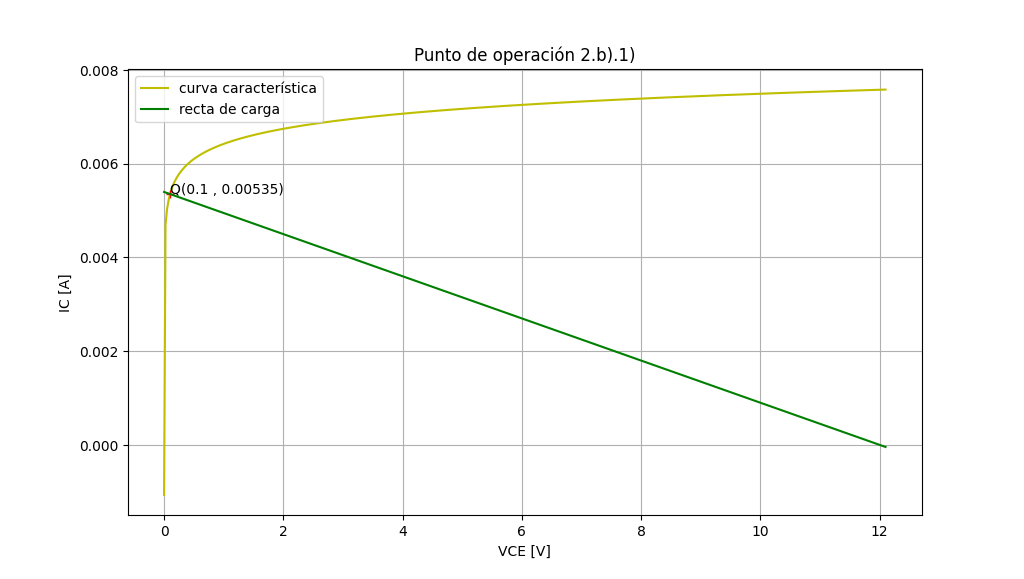
\includegraphics[height=5cm\textwidth]{2b1.png}
        \caption{Curva Característica, recta de carga y punto de operación del circuito de la figura \ref{fig:10}, con valores de resistencias expresados en \ref{tab:2b1}}
        \label{fig:2b1}
    \end{figure}

    \newpage

    \begin{table}[h!]
        \centering
        \caption{Valores de resistencia para la prueba de laboratorio \ref{pru3}}
        \label{tab:2b2}
        \begin{tabular}{|c|c|c|} \hline
            RB & RC & RE \\ \hline
            $36k\Omega \pm 10\%$ & $2k\Omega \pm 10\%$ & $200\Omega \pm 10\%$ \\ \hline
        \end{tabular}
    \end{table}

    \begin{figure}[h!]
        \centering
        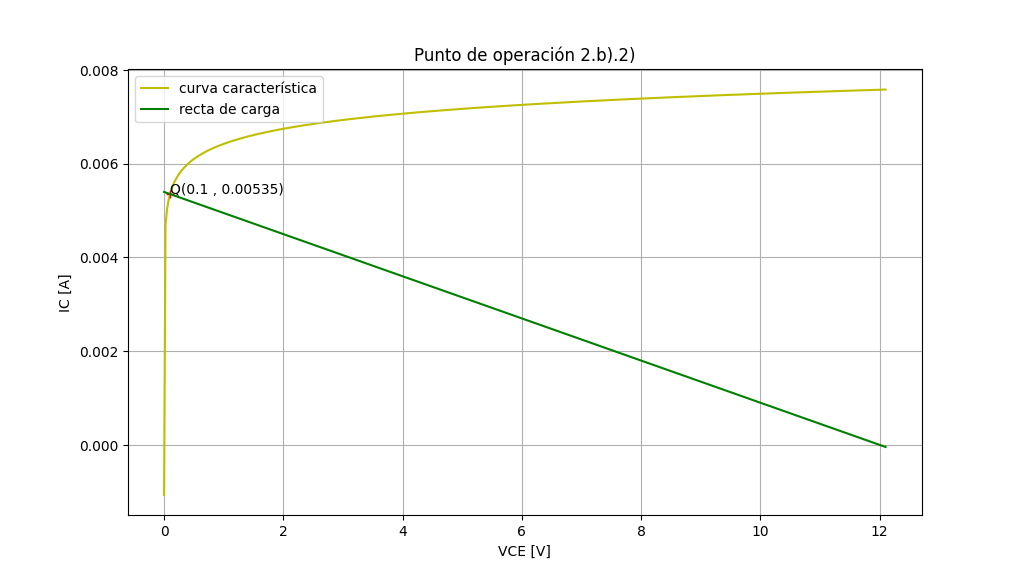
\includegraphics[height=5cm\textwidth]{2b2.png}
        \caption{Curva Característica, recta de carga y punto de operación del circuito de la figura \ref{fig:10}, con valores de resistencias expresados en \ref{tab:2b2}}
        \label{fig:2b2}
    \end{figure}
    
    \begin{table}[h!]
        \centering
        \caption{Valores de resistencia para la prueba de laboratorio \ref{pru4}}
        \label{tab:2b3}
        \begin{tabular}{|c|c|c|} \hline
            RB & RC & RE \\ \hline
            $56k\Omega \pm 10\%$ & $3k\Omega \pm 10\%$ & $200\Omega \pm 10\%$ \\ \hline
        \end{tabular}
    \end{table}

    \begin{figure}[h!]
        \centering
        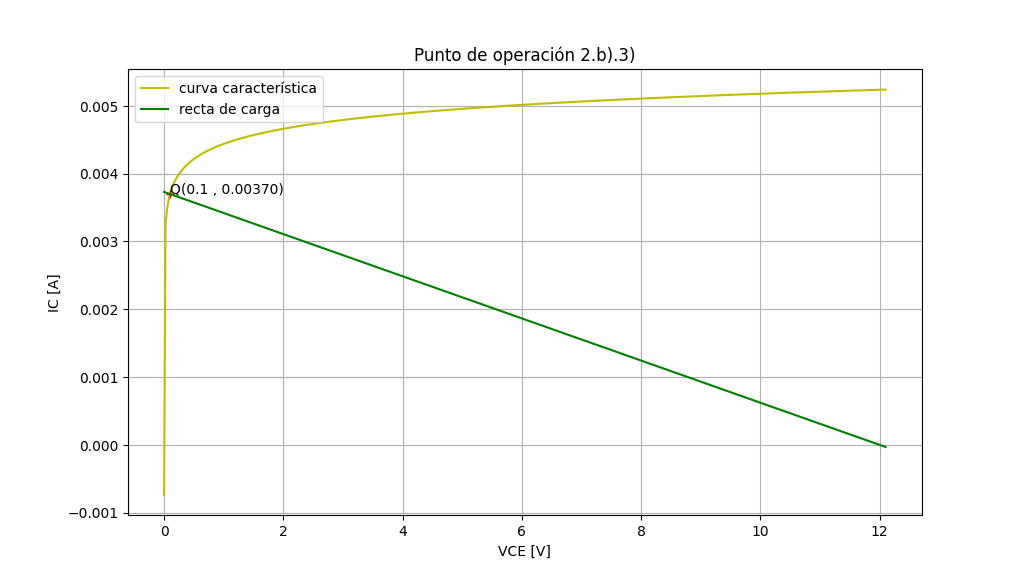
\includegraphics[height=5cm\textwidth]{2b3.png}
        \caption{Curva Característica, recta de carga y punto de operación del circuito de la figura \ref{fig:10}, con valores de resistencias expresados en \ref{tab:2b3}}
        \label{fig:2b3}
    \end{figure}

    \newpage

    \begin{table}[h!]
        \centering
        \caption{Valores de resistencia para la prueba de laboratorio \ref{pru5}}
        \label{tab:2b4}
        \begin{tabular}{|c|c|c|} \hline
            RB & RC & RE \\ \hline
            $56k\Omega \pm 10\%$ & $1,3k\Omega \pm 10\%$ & $200\Omega \pm 10\%$ \\ \hline
        \end{tabular}
    \end{table}

    \begin{figure}[h!]
        \centering
        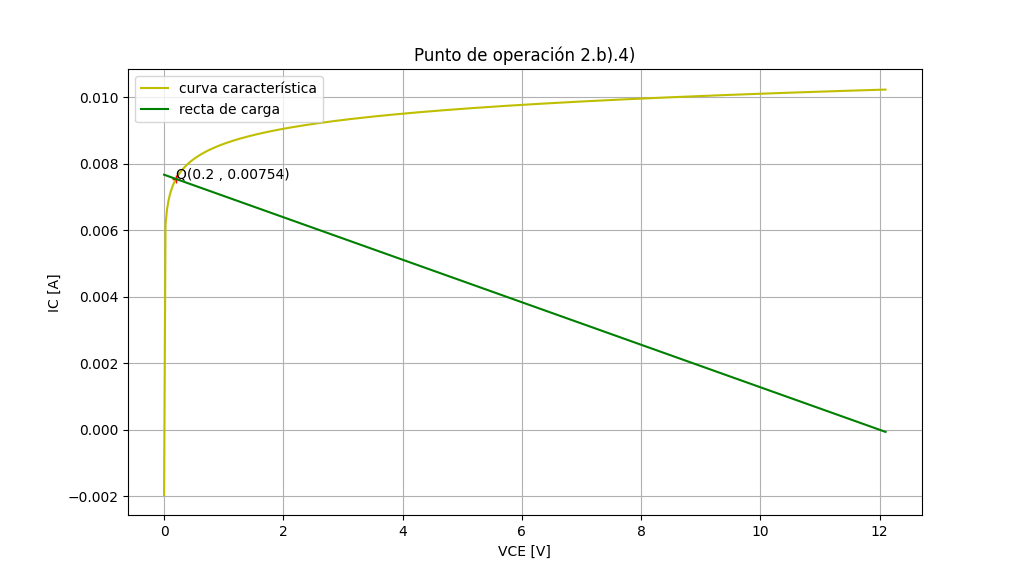
\includegraphics[height=5cm\textwidth]{2b4.png}
        \caption{Curva Característica, recta de carga y punto de operación del circuito de la figura \ref{fig:10}, con valores de resistencias expresados en \ref{tab:2b4}}
        \label{fig:2b4}
    \end{figure}

    \begin{table}[h!]
        \centering
        \caption{Valores de resistencia para la prueba de laboratorio \ref{pru6}}
        \label{tab:2b5}
        \begin{tabular}{|c|c|c|} \hline
            RB & RC & RE \\ \hline
            $56k\Omega \pm 10\%$ & $2k\Omega \pm 10\%$ & $300\Omega \pm 10\%$ \\ \hline
        \end{tabular}
    \end{table}

    \begin{figure}[h!]
        \centering
        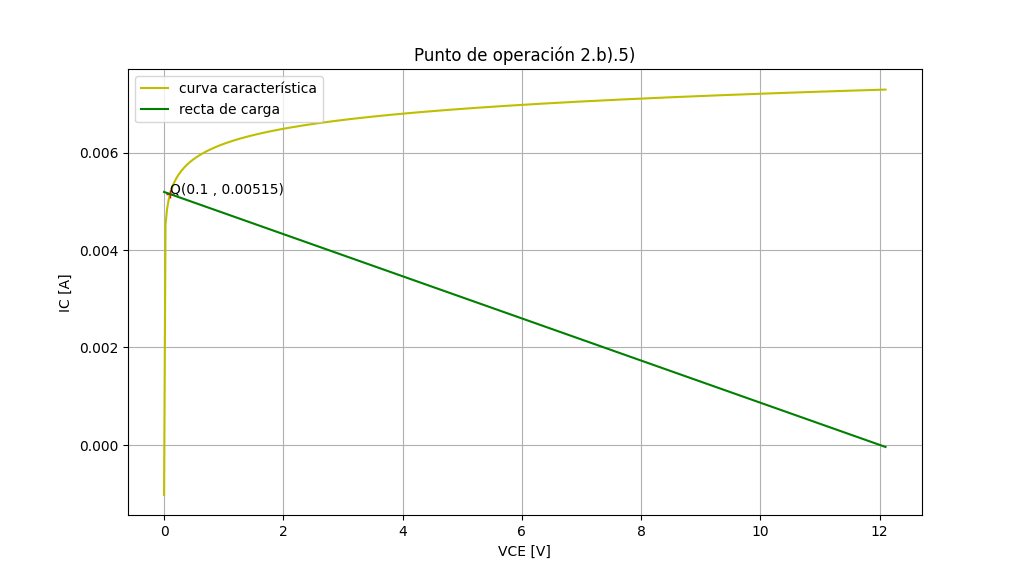
\includegraphics[height=5cm\textwidth]{2b5.png}
        \caption{Curva Característica, recta de carga y punto de operación del circuito de la figura \ref{fig:10}, con valores de resistencias expresados en \ref{tab:2b5}}
        \label{fig:2b5}
    \end{figure}

    \newpage

    \begin{table}[h!]
        \centering
        \caption{Valores de resistencia para la prueba de laboratorio \ref{pru7}}
        \label{tab:2b6}
        \begin{tabular}{|c|c|c|} \hline
            RB & RC & RE \\ \hline
            $56k\Omega \pm 10\%$ & $2k\Omega \pm 10\%$ & $130\Omega \pm 10\%$ \\ \hline
        \end{tabular}
    \end{table}

    \begin{figure}[h!]
        \centering
        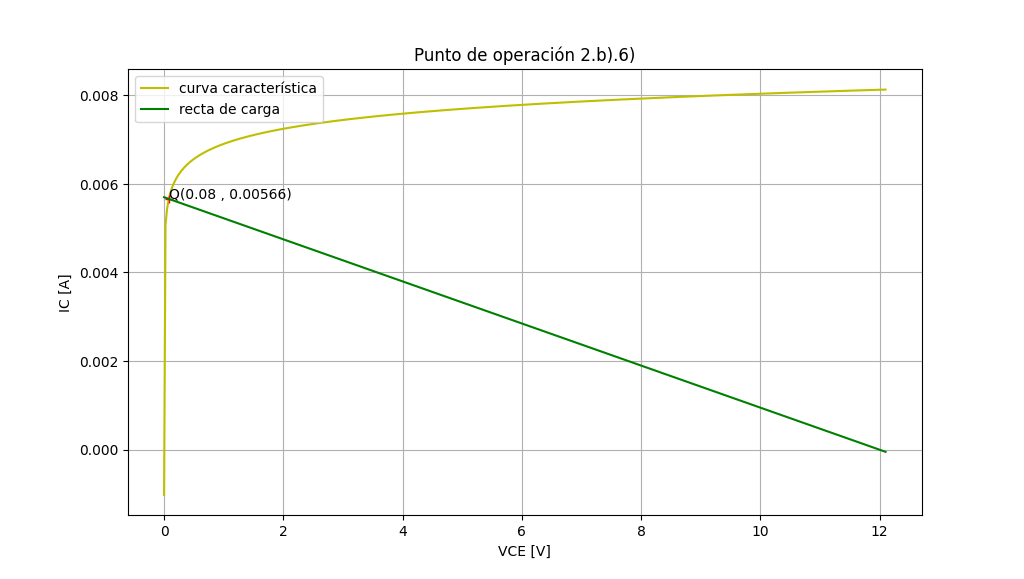
\includegraphics[height=5cm\textwidth]{2b6.png}
        \caption{Curva Característica, recta de carga y punto de operación del circuito de la figura \ref{fig:10}, con valores de resistencias expresados en \ref{tab:2b6}}
        \label{fig:2b6}
    \end{figure}

    \begin{table}[h!]
        \centering
        \caption{Valores de resistencia para la prueba de laboratorio \ref{pru8}}
        \label{tab:3a}
        \begin{tabular}{|c|c|c|c|} \hline
            R1 & R2 & RC & RE \\ \hline
            $56k\Omega \pm 10\%$ & $10k\Omega \pm 10\%$ & $510\Omega \pm 10\%$ & $200\Omega \pm 10\%$ \\ \hline
        \end{tabular}
    \end{table}

    \begin{figure}[h!]
        \centering
        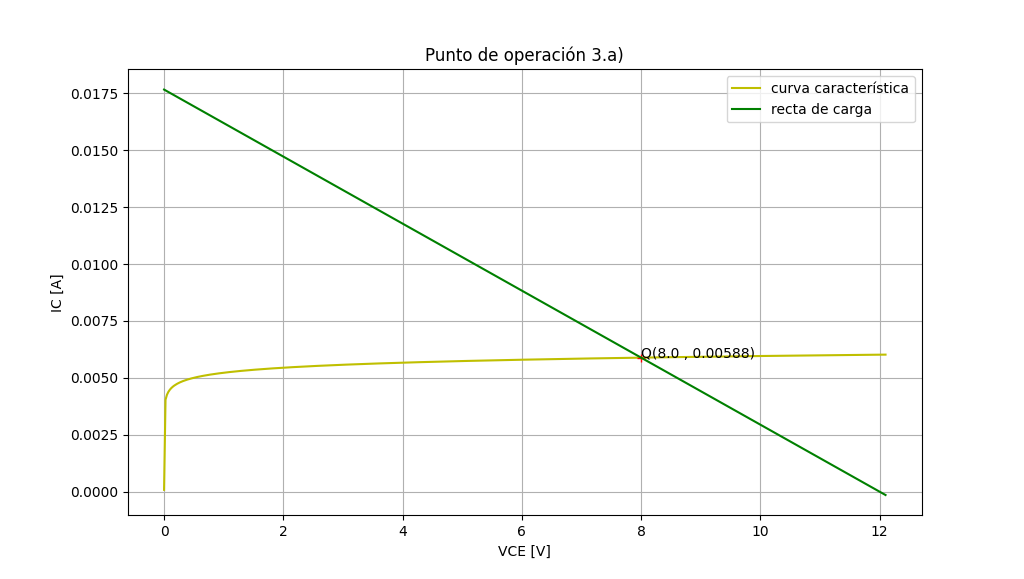
\includegraphics[height=5cm\textwidth]{3a.png}
        \caption{Curva Característica, recta de carga y punto de operación del circuito de la figura \ref{fig:11}, con valores de resistencias expresados en \ref{tab:3a}}
        \label{fig:3a}
    \end{figure}

    \newpage

    \begin{table}[h!]
        \centering
        \caption{Valores de resistencia para la prueba de laboratorio \ref{pru9}}
        \label{tab:3b1}
        \begin{tabular}{|c|c|c|c|} \hline
            R1 & R2 & RC & RE \\ \hline
            $82k\Omega \pm 10\%$ & $10k\Omega \pm 10\%$ & $510\Omega \pm 10\%$ & $200\Omega \pm 10\%$ \\ \hline
        \end{tabular}
    \end{table}

    \begin{figure}[h!]
        \centering
        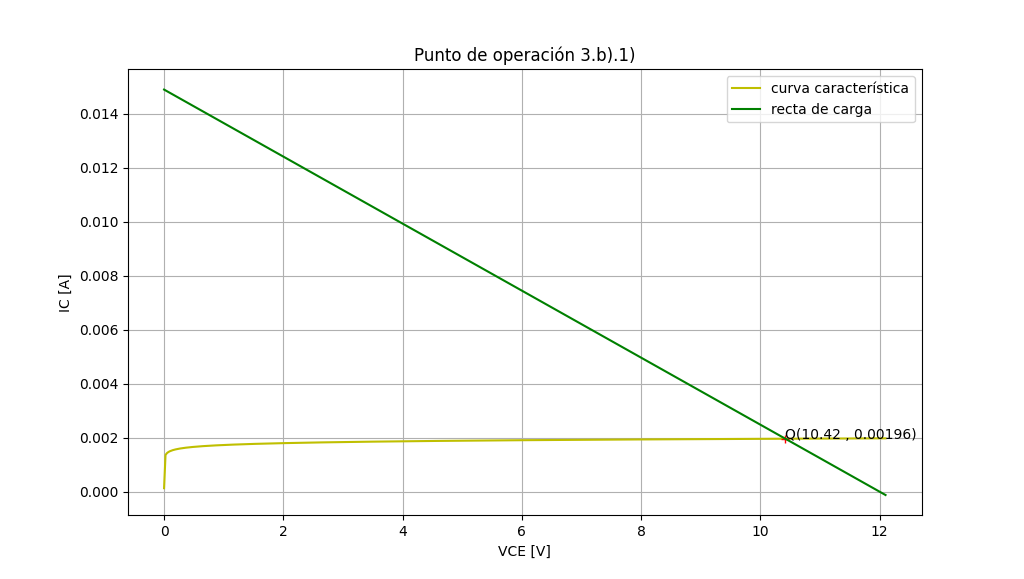
\includegraphics[height=5cm\textwidth]{3b1.png}
        \caption{Curva Característica, recta de carga y punto de operación del circuito de la figura \ref{fig:11}, con valores de resistencias expresados en \ref{tab:3b1}}
        \label{fig:3b1}
    \end{figure}

    \begin{table}[h!]
        \centering
        \caption{Valores de resistencia para la prueba de laboratorio \ref{pru10}}
        \label{tab:3b2}
        \begin{tabular}{|c|c|c|c|} \hline
            R1 & R2 & RC & RE \\ \hline
            $39k\Omega \pm 10\%$ & $10k\Omega \pm 10\%$ & $510\Omega \pm 10\%$ & $200\Omega \pm 10\%$ \\ \hline
        \end{tabular}
    \end{table}

    \begin{figure}[h!]
        \centering
        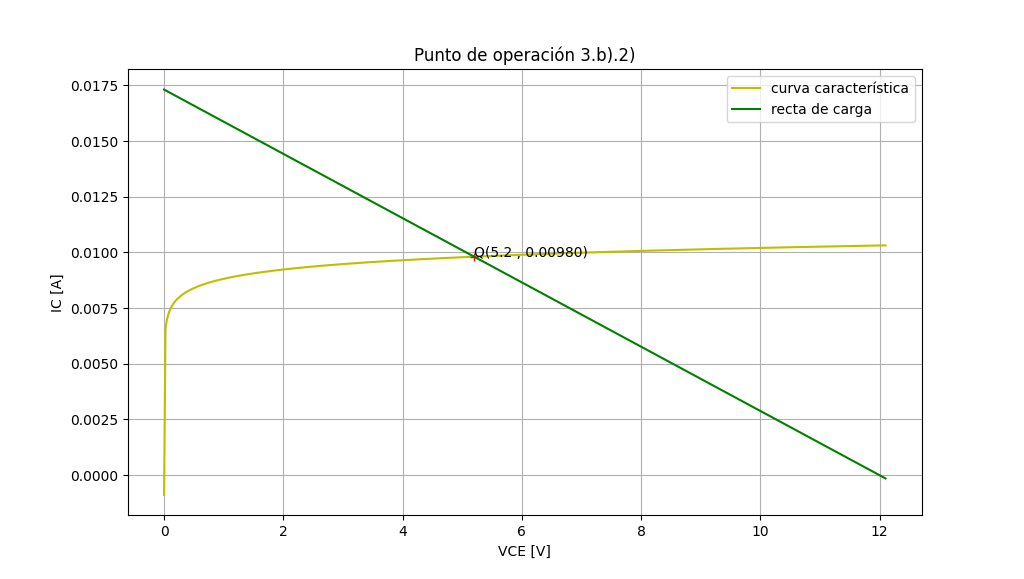
\includegraphics[height=5cm\textwidth]{3b2.png}
        \caption{Curva Característica, recta de carga y punto de operación del circuito de la figura \ref{fig:11}, con valores de resistencias expresados en \ref{tab:3b2}}
        \label{fig:3b2}
    \end{figure}

    \newpage

    \begin{table}[h!]
        \centering
        \caption{Valores de resistencia para la prueba de laboratorio \ref{pru11}}
        \label{tab:3b3}
        \begin{tabular}{|c|c|c|c|} \hline
            R1 & R2 & RC & RE \\ \hline
            $56k\Omega \pm 10\%$ & $15k\Omega \pm 10\%$ & $510\Omega \pm 10\%$ & $200\Omega \pm 10\%$ \\ \hline
        \end{tabular}
    \end{table}

    \begin{figure}[h!]
        \centering
        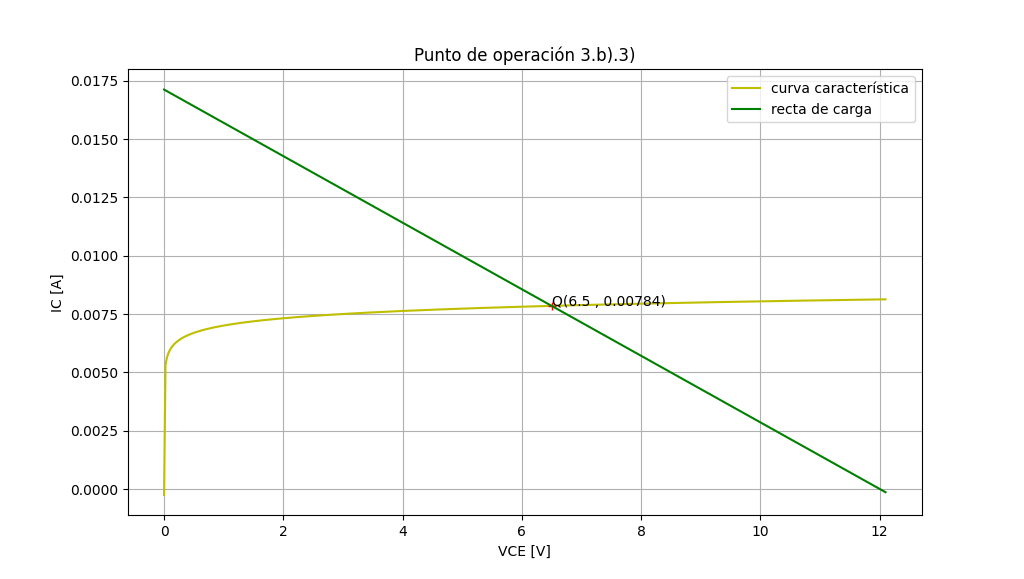
\includegraphics[height=5cm\textwidth]{3b3.png}
        \caption{Curva Característica, recta de carga y punto de operación del circuito de la figura \ref{fig:11}, con valores de resistencias expresados en \ref{tab:3b3}}
        \label{fig:3b3}
    \end{figure}

    \begin{table}[h!]
        \centering
        \caption{Valores de resistencia para la prueba de laboratorio \ref{pru12}}
        \label{tab:3b4}
        \begin{tabular}{|c|c|c|c|} \hline
            R1 & R2 & RC & RE \\ \hline
            $56k\Omega \pm 10\%$ & $6,8k\Omega \pm 10\%$ & $510\Omega \pm 10\%$ & $200\Omega \pm 10\%$ \\ \hline
        \end{tabular}
    \end{table}

    \begin{figure}[h!]
        \centering
        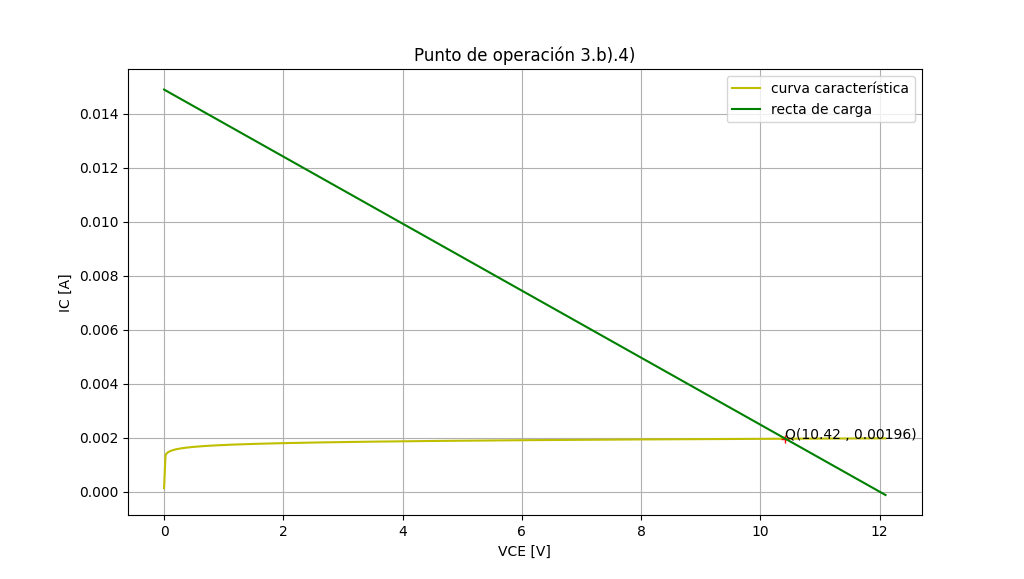
\includegraphics[height=5cm\textwidth]{3b4.png}
        \caption{Curva Característica, recta de carga y punto de operación del circuito de la figura \ref{fig:11}, con valores de resistencias expresados en \ref{tab:3b4}}
        \label{fig:3b4}
    \end{figure}

    \newpage

    \begin{table}[h!]
        \centering
        \caption{Valores de resistencia para la prueba de laboratorio \ref{pru13}}
        \label{tab:3b5}
        \begin{tabular}{|c|c|c|c|} \hline
            R1 & R2 & RC & RE \\ \hline
            $56k\Omega \pm 10\%$ & $56k\Omega \pm 10\%$ & $750\Omega \pm 10\%$ & $200\Omega \pm 10\%$ \\ \hline
        \end{tabular}
    \end{table}

    \begin{figure}[h!]
        \centering
        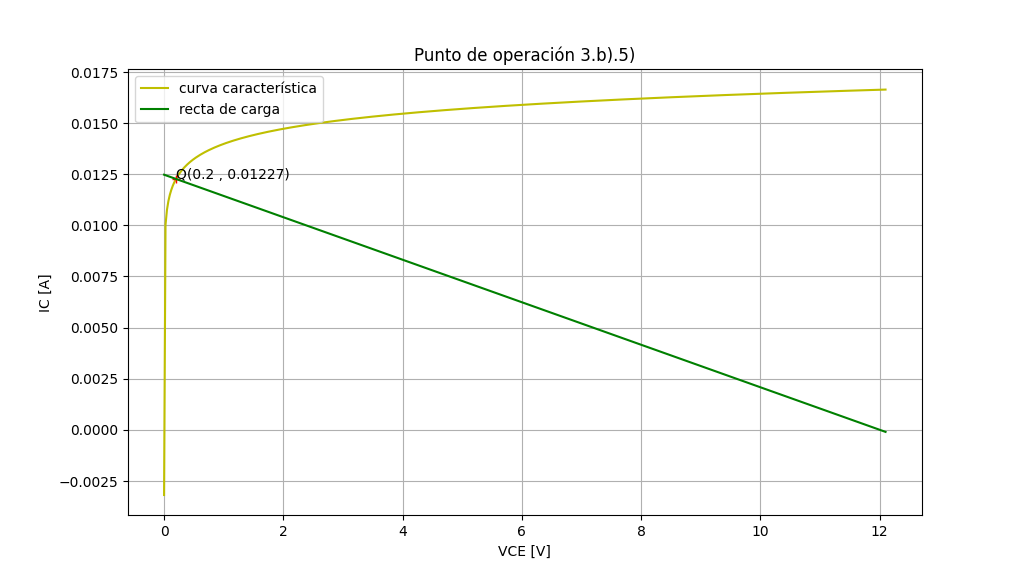
\includegraphics[height=5cm\textwidth]{3b5.png}
        \caption{Curva Característica, recta de carga y punto de operación del circuito de la figura \ref{fig:11}, con valores de resistencias expresados en \ref{tab:3b5}}
        \label{fig:3b5}
    \end{figure}

    \begin{table}[h!]
        \centering
        \caption{Valores de resistencia para la prueba de laboratorio \ref{pru14}}
        \label{tab:3b6}
        \begin{tabular}{|c|c|c|c|} \hline
            R1 & R2 & RC & RE \\ \hline
            $56k\Omega \pm 10\%$ & $56k\Omega \pm 10\%$ & $360\Omega \pm 10\%$ & $200\Omega \pm 10\%$ \\ \hline
        \end{tabular}
    \end{table}

    \begin{figure}[h!]
        \centering
        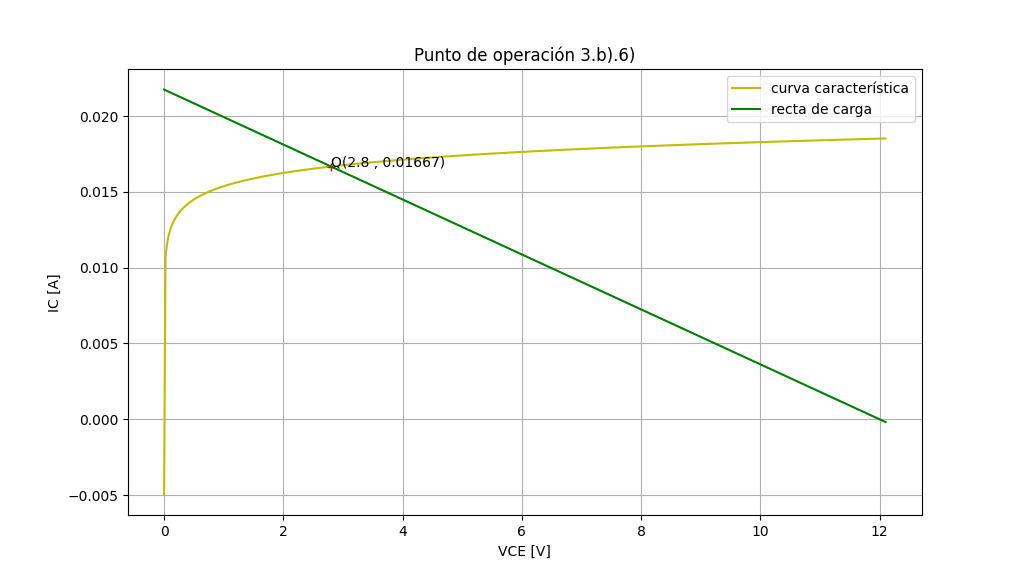
\includegraphics[height=5cm\textwidth]{3b6.png}
        \caption{Curva Característica, recta de carga y punto de operación del circuito de la figura \ref{fig:11}, con valores de resistencias expresados en \ref{tab:3b6}}
        \label{fig:3b6}
    \end{figure}

    \newpage

    \begin{figure}[h!]
        \centering
        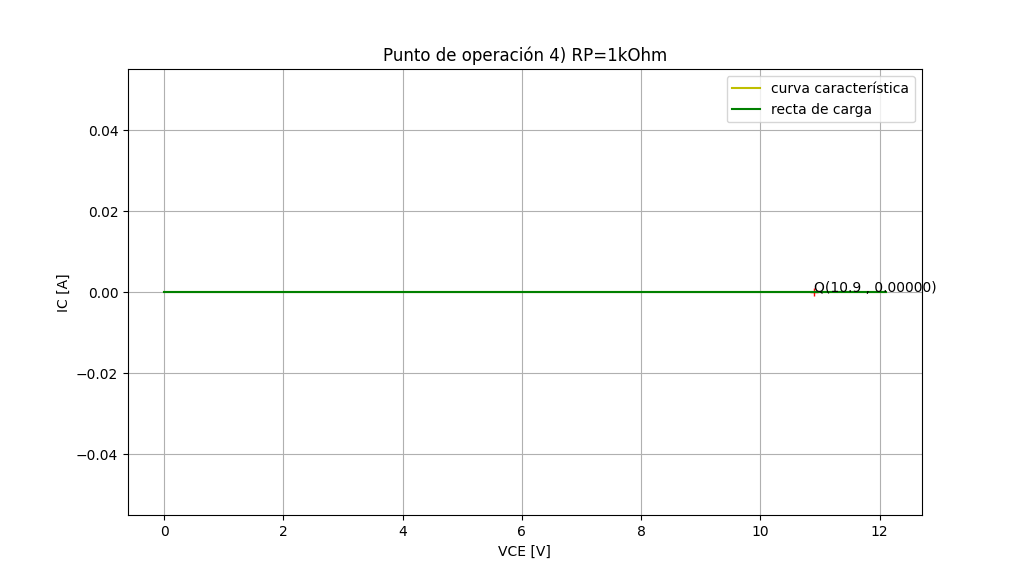
\includegraphics[height=5cm\textwidth]{4RP1K.png}
        \caption{Curva Característica, recta de carga y punto de operación del circuito de la figura \ref{fig:12}, con $RP = 1K\Omega$}
        \label{fig:4RP1K}
    \end{figure}

    \begin{figure}[h!]
        \centering
        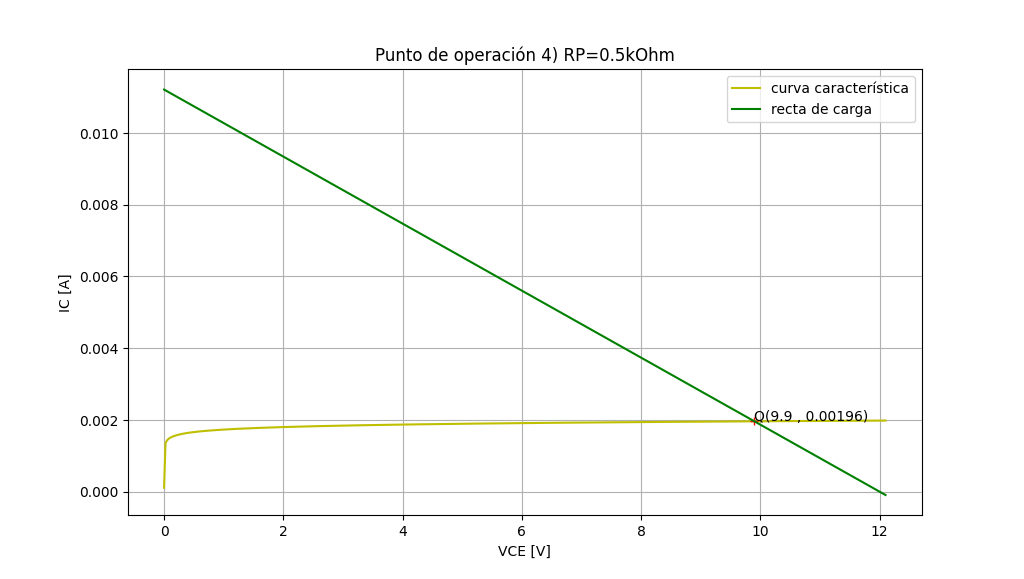
\includegraphics[height=5cm\textwidth]{4RP05K.png}
        \caption{Curva Característica, recta de carga y punto de operación del circuito de la figura \ref{fig:12}, con $RP = 0.5K\Omega$}
        \label{fig:4RP05K}
    \end{figure}

    \begin{figure}[h!]
        \centering
        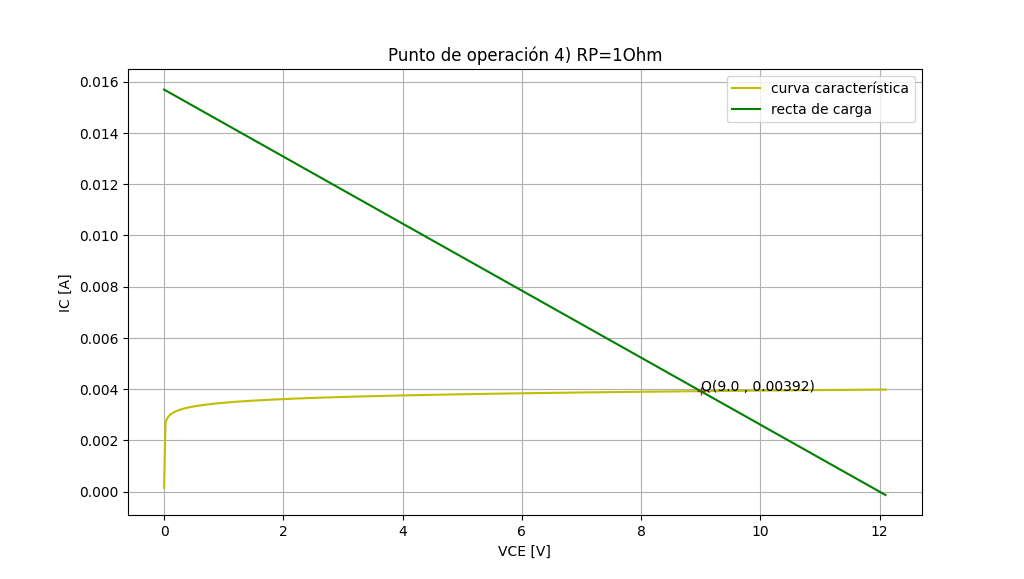
\includegraphics[height=5cm\textwidth]{4RP1.png}
        \caption{Curva Característica, recta de carga y punto de operación del circuito de la figura \ref{fig:12}, con $RP = 1\Omega$}
        \label{fig:4RP1}
    \end{figure}

    \newpage

    \section{Análisis de Resultados}

    En la tabla \ref{tab:1} es notable que los puntos de operación estáticos experimentales de los circuitos \ref{fig:7} y \ref{fig:8} son iguales a los ya calculados teóricamente en \ref{tab:Qt}. En particular, cabe señalar que esto es debido a la ausencia de polarización en la unión base-emisor del transistor. No obstante, el punto estático de operación de la tabla \ref{tab:1} para el circuito de la figura \ref{fig:9} no coincide con los valores teóricos de la otra tabla mencionada, sin embargo, al recordar que, teóricamente, se obtuvo una tensión colector emisor alta en módulo y negativa; y observando la gráfica \ref{fig:1cir3} donde la tensión alcanza un valor sumante bajo, se puede decir que el transistor se encuentra saturado. Esto último debido a que, a diferencia de los circuitos anteriores existe una polarización directa en la unión base emisor.

    Para el circuito de la figura \ref{fig:10} el punto de operación estático tiene un comportamiento similar que el del circuito de la figura \ref{fig:9}, ya explicado en el párrafo anterior. Por añadidura de RE y observando la gráfica  \ref{fig:2a} el transistor se encuentra saturado, aunque es notable que la $V_{CE}$ incrementó 10mV.

    Al analizar la figura \ref{fig:11} y comparando el primer valor de la tabla \ref{tab:3} y el $Q_5$ de la tabla \ref{tab:Qt} es notable que se realizó una buena aproximación del punto estático de operación, vinculado a la zona activa del transistor, con un error que puede estar relacionado a la toma del valor $h_{FE}$ por debajo de lo establecido por la condiciones del circuito planteado, esto se deduce debido a que la gráfica \ref{fig:3a} posee un Q con una intensidad de colector de poco más de 5mA, mayor que la calculada teóricamente.

    Cabe destacar en la figura \ref{fig:10} que al calcular los puntos de operación estáticos referente al trabajo de laboratorio \ref{i2}, todos quedaron vinculados a la zona de saturación, esto debido a que tiene un comportamiento de polarización solamente, semejante a lo ocurrido con el Q de la figura \ref{fig:9}, ocasiones leves variaciones en la corriente de colector que entran en el rango de los 3.70 mA hasta los 7.53 mA, donde existe una media de 5.44 mA que se mantiene en las pruebas. Sin embargo, se hace notar en la prueba \ref{pru5} un cambio poco significativo que tiende a la zona activa, sin llegar a acercarse lo suficiente como para que el transistor trabaje en la zona activa. Las gráficas que representan el comportamiento del circuito se asocian a las figuras desde la \ref{fig:2b1} hasta \ref{fig:2b6}.

    En el circuito de la figura \ref{fig:11} se puede generalizar que los puntos de operación estáticos se encuentran en la zona activa de la curva característica del transistor o entre sus límites, según la tabla \ref{tab:3}, sin importar las distintas variaciones de resistencias, que según la aplicación del transistor de puede modificar Q de manera que tienda a la zona de corte o saturación. Este hecho es debido a la presencia de R2 en el circuito comparado con el anterior. No obstante, para particularizar cuando R1 Y R2 son altas respecto a los valores de RC y RE, como es el caso de las pruebas \ref{pru13} y \ref{pru14} el transistor trabaja casi en zona de saturación; también se observa en las pruebas donde R1 es sumamente alta con respecto a las demás resistencias que el transistor puede llegar a corte, esto debido a la poca tensión que se obtendría entre base y emisor, siendo el caso de las pruebas \ref{pru9} y \ref{pru12}. Las gráficas que representan el comportamiento del circuito se asocian a las figuras desde la \ref{fig:3b1} hasta \ref{fig:3b6}.

    Por último, para estudiar el efecto de la resistencia equivalente en el emisor se implementó la figura \ref{fig:12}, donde al poseer una $RE_{eq}$ alta el transistor, como en la prueba 1 de la tabla \ref{tab:4} se encuentra en zona de corte, lo cual tiene sentido ya que se sabe $I_E = I_C + I_B$ que es la corriente neta que circula por el transistor, al limitarla el punto de operación desciende a $I_C = 0$. Al ir disminuyendo la resistencia RP en el emisor el transistor tiende a operar en la zona activa, notable en las gráficas de las figura \ref{fig:4RP1K}, \ref{fig:4RP05K} y \ref{fig:4RP1}.

    \newpage

    \section{Conclusiones y Recomendaciones}

    Este laboratorio nos ha permitido conocer y comparar las distintas topologías para polarizar un BJT, así como los factores que influyen en su punto de operación. Conocer el punto de operación de un transistor es importante porque determina el comportamiento y el rendimiento del transistor en un circuito. El punto de operación es el conjunto de valores de corriente y tensión que el transistor tiene cuando no se aplica ninguna señal de entrada. Este punto se puede ubicar en diferentes regiones del transistor, como la de corte, la de saturación o la de activa, según el tipo de aplicación que se le quiera dar al transistor. También se ha observado que algunas topologías son más estables que otras, y que el valor de las resistencias de base, colector y emisor determina la posición del punto de operación sobre la recta de carga y la característica del transistor.
    
    Se puede observar que algunas topologías son más sensibles a las variaciones de las resistencias, lo que puede llevar al transistor a zonas no deseadas, como la de corte o la de saturación, dependiendo de su aplicación. También se ha analizado cómo las resistencias de base, colector y emisor modifican la recta de carga y la posición del punto de operación sobre la característica del transistor. La recta de carga estática en un transistor es importante porque permite determinar el punto de operación del transistor en la región activa, donde el transistor puede amplificar correctamente la señal de entrada sin distorsiones. La recta de carga estática representa todos los posibles puntos de polarización que el circuito externo le impone al transistor, y se puede graficar sobre las curvas características del transistor. La posición del punto de operación sobre la recta de carga estática depende de los valores de las resistencias y la fuente de alimentación del circuito de polarización. También se ha aprendido que se pueden diseñar circuitos que cumpla con nuestros requisitos, eligiendo adecuadamente los valores de las resistencias y los parámetros del transistor, como β y VBE. También se ha comprobado que los resultados experimentales se ajustan bastante a los resultados teóricos, lo que nos indica que el modelo teórico es válido y que hemos realizado las mediciones correctamente.

    \newpage

    \section{Bibliografía}

    \printbibliography

    \newpage

    \section{Anexos}

    Para el cálculo del punto de operación en las tablas \ref{tab:1}, \ref{tab:2}, \ref{tab:3} y \ref{tab:4}:

    Sabiendo que $V_{CC} = 12 \pm 1 [V]$

    \setcounter{equation}{1}
    \begin{equation}
        V_{CE} = V_C - V_E
        \label{Qeq1}
    \end{equation}

    \setcounter{equation}{1}
    \begin{equation}
        I_C = \frac{V_{CC} - V_C}{R_C}
        \label{Qeq2}
    \end{equation}

    Para el cálculo de sus respectivas incertidumbres:

    \setcounter{equation}{1}
    \begin{equation}
        \Delta V_{CE} = \Delta V_C + \Delta V_E
        \label{Qeq3}
    \end{equation}

    \begin{equation}
        \begin{split}
            \Delta I_C & = \left | \frac{\partial I_C}{\partial V_{CC}} \right | \Delta V_{CC} + \left | \frac{\partial I_C}{\partial V_C} \right | \Delta V_C + \left | \frac{\partial I_C}{\partial R_C} \right | \Delta R_C \\
            & = {1 \over R_C} \Delta V_{CC} + {1 \over R_C} \Delta V_C + \frac{V_{CC}-V_C}{R_C^2} \Delta R_C
        \end{split}
        \label{Qeq4}
    \end{equation}

    \newpage

    Hojas de datos que contienen los valores experimentales recopilados en el laboratorio.

    \begin{figure}
        \centering
        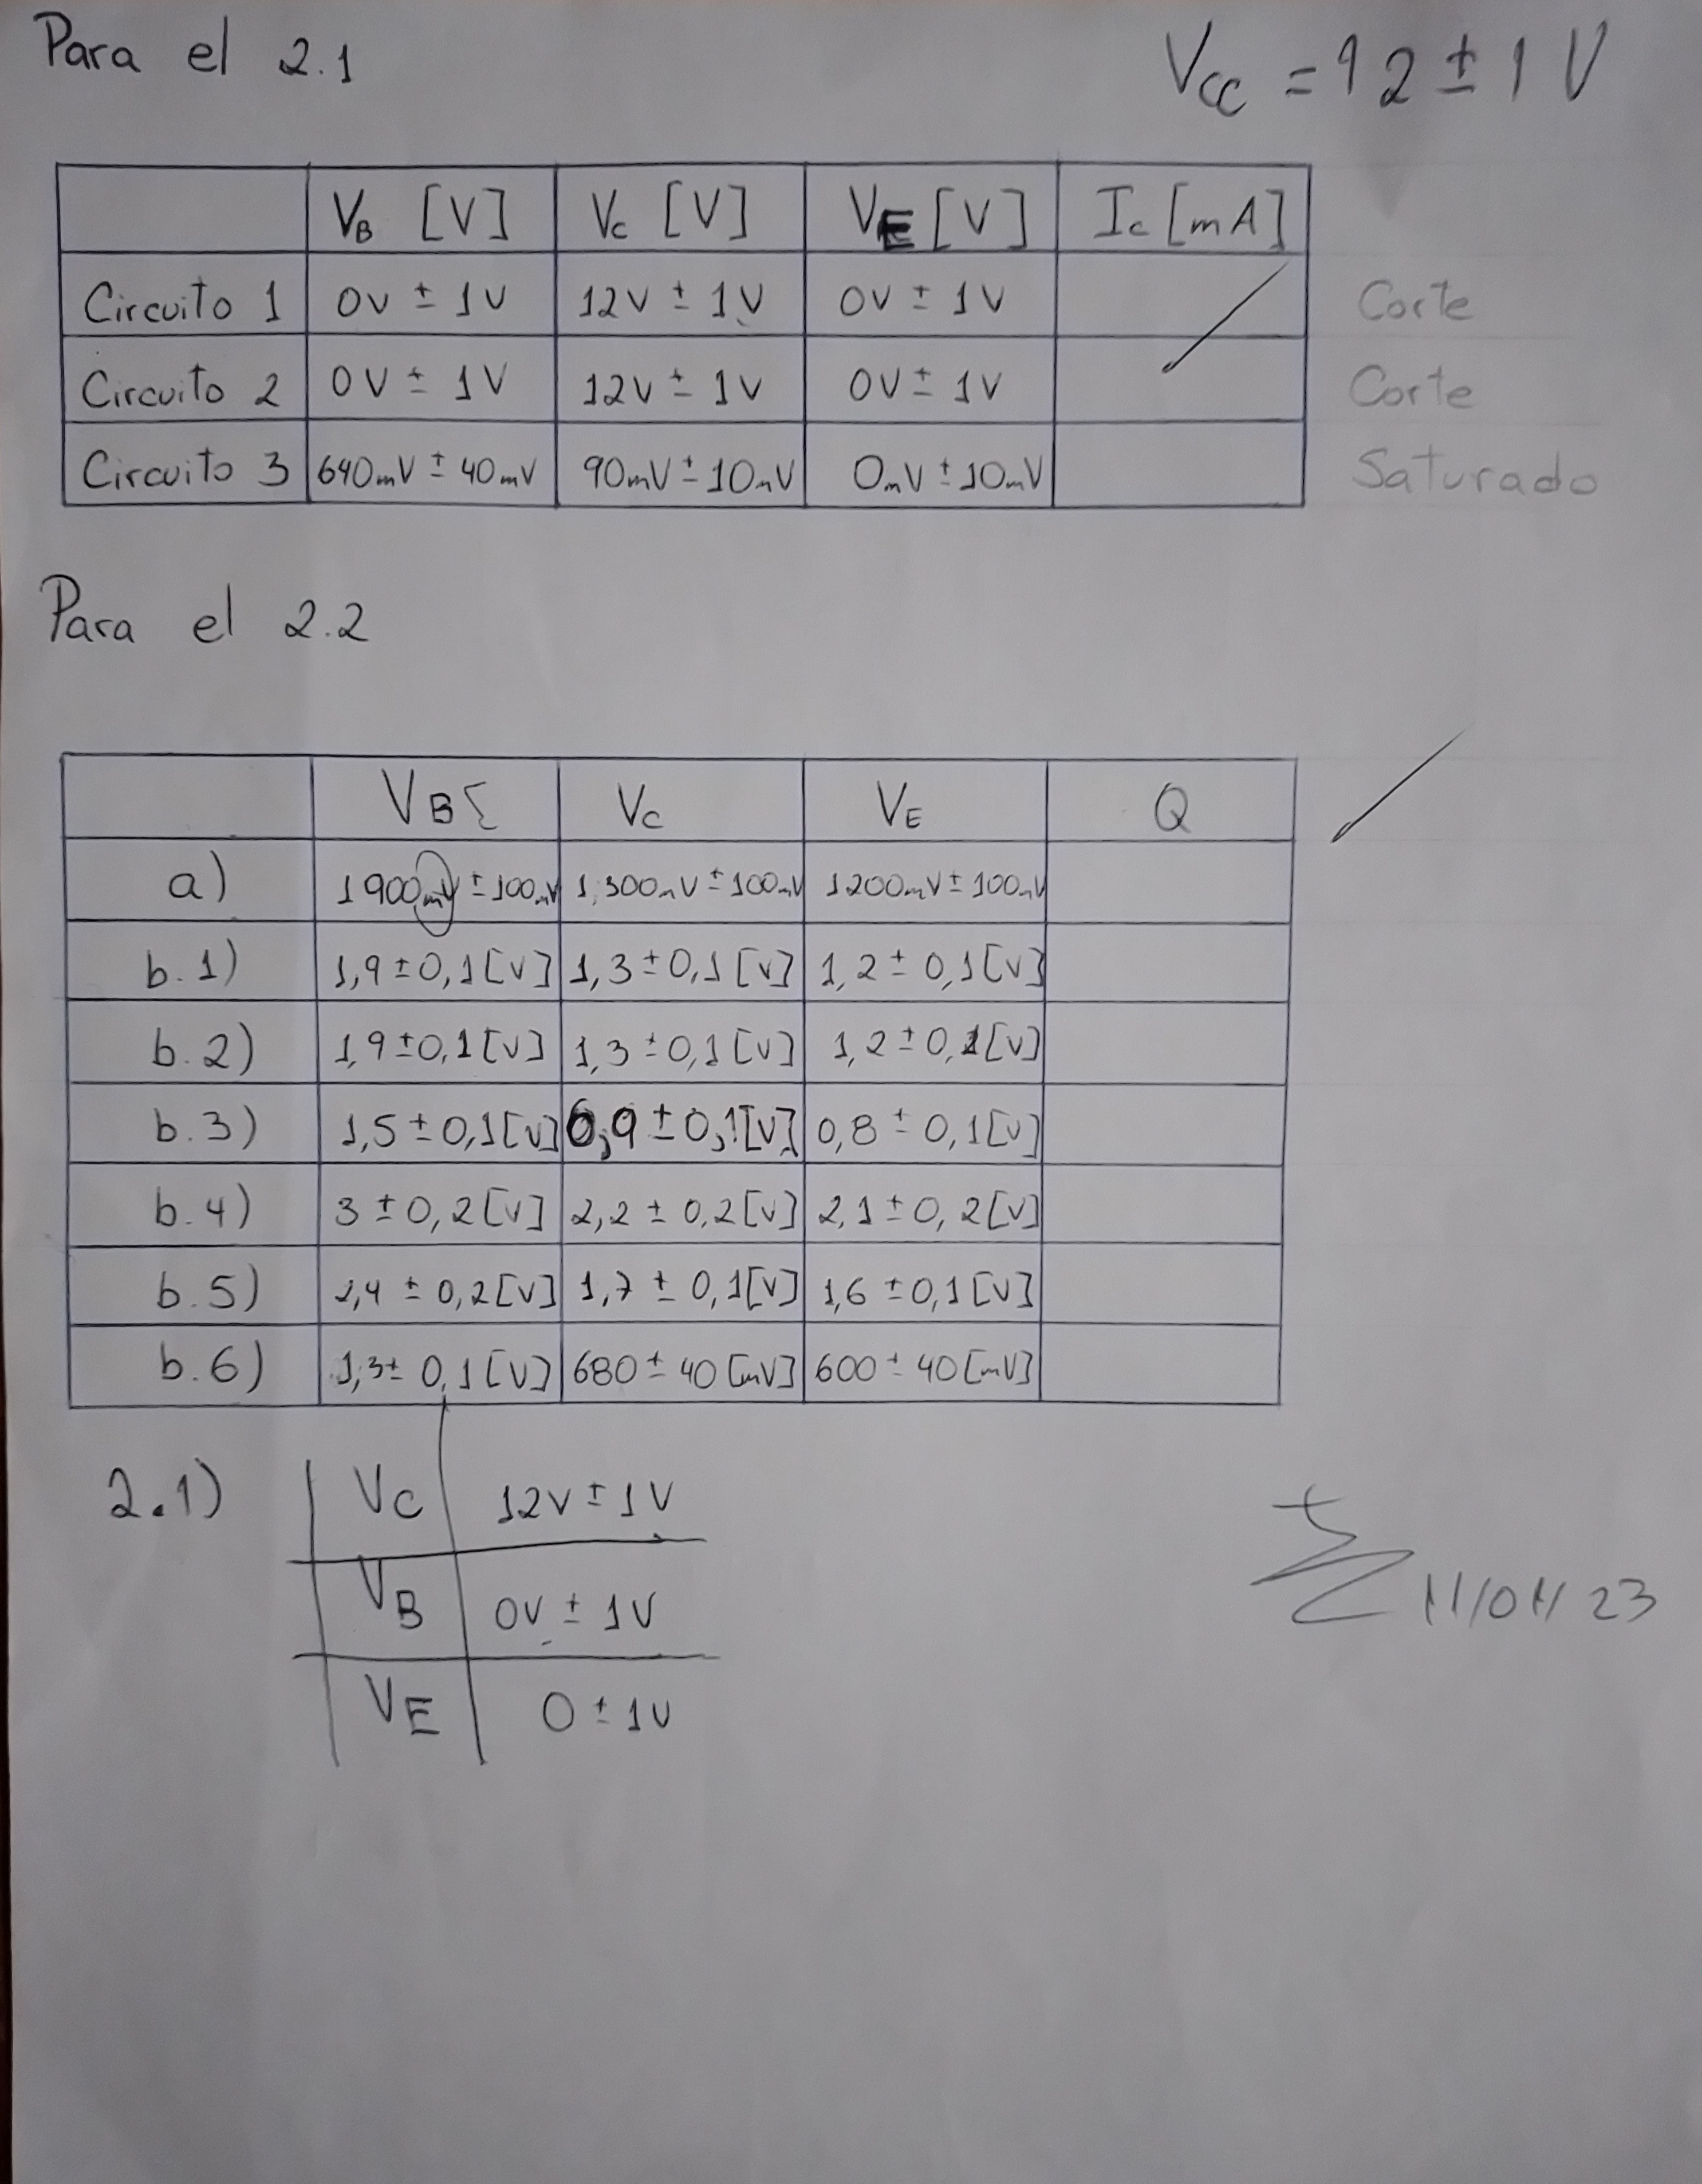
\includegraphics[height=10cm\textwidth]{hojadatos1.jpg}
        \caption{hoja de datos 1}
        \label{fig:hd1}
    \end{figure}

    \begin{figure}
        \centering
        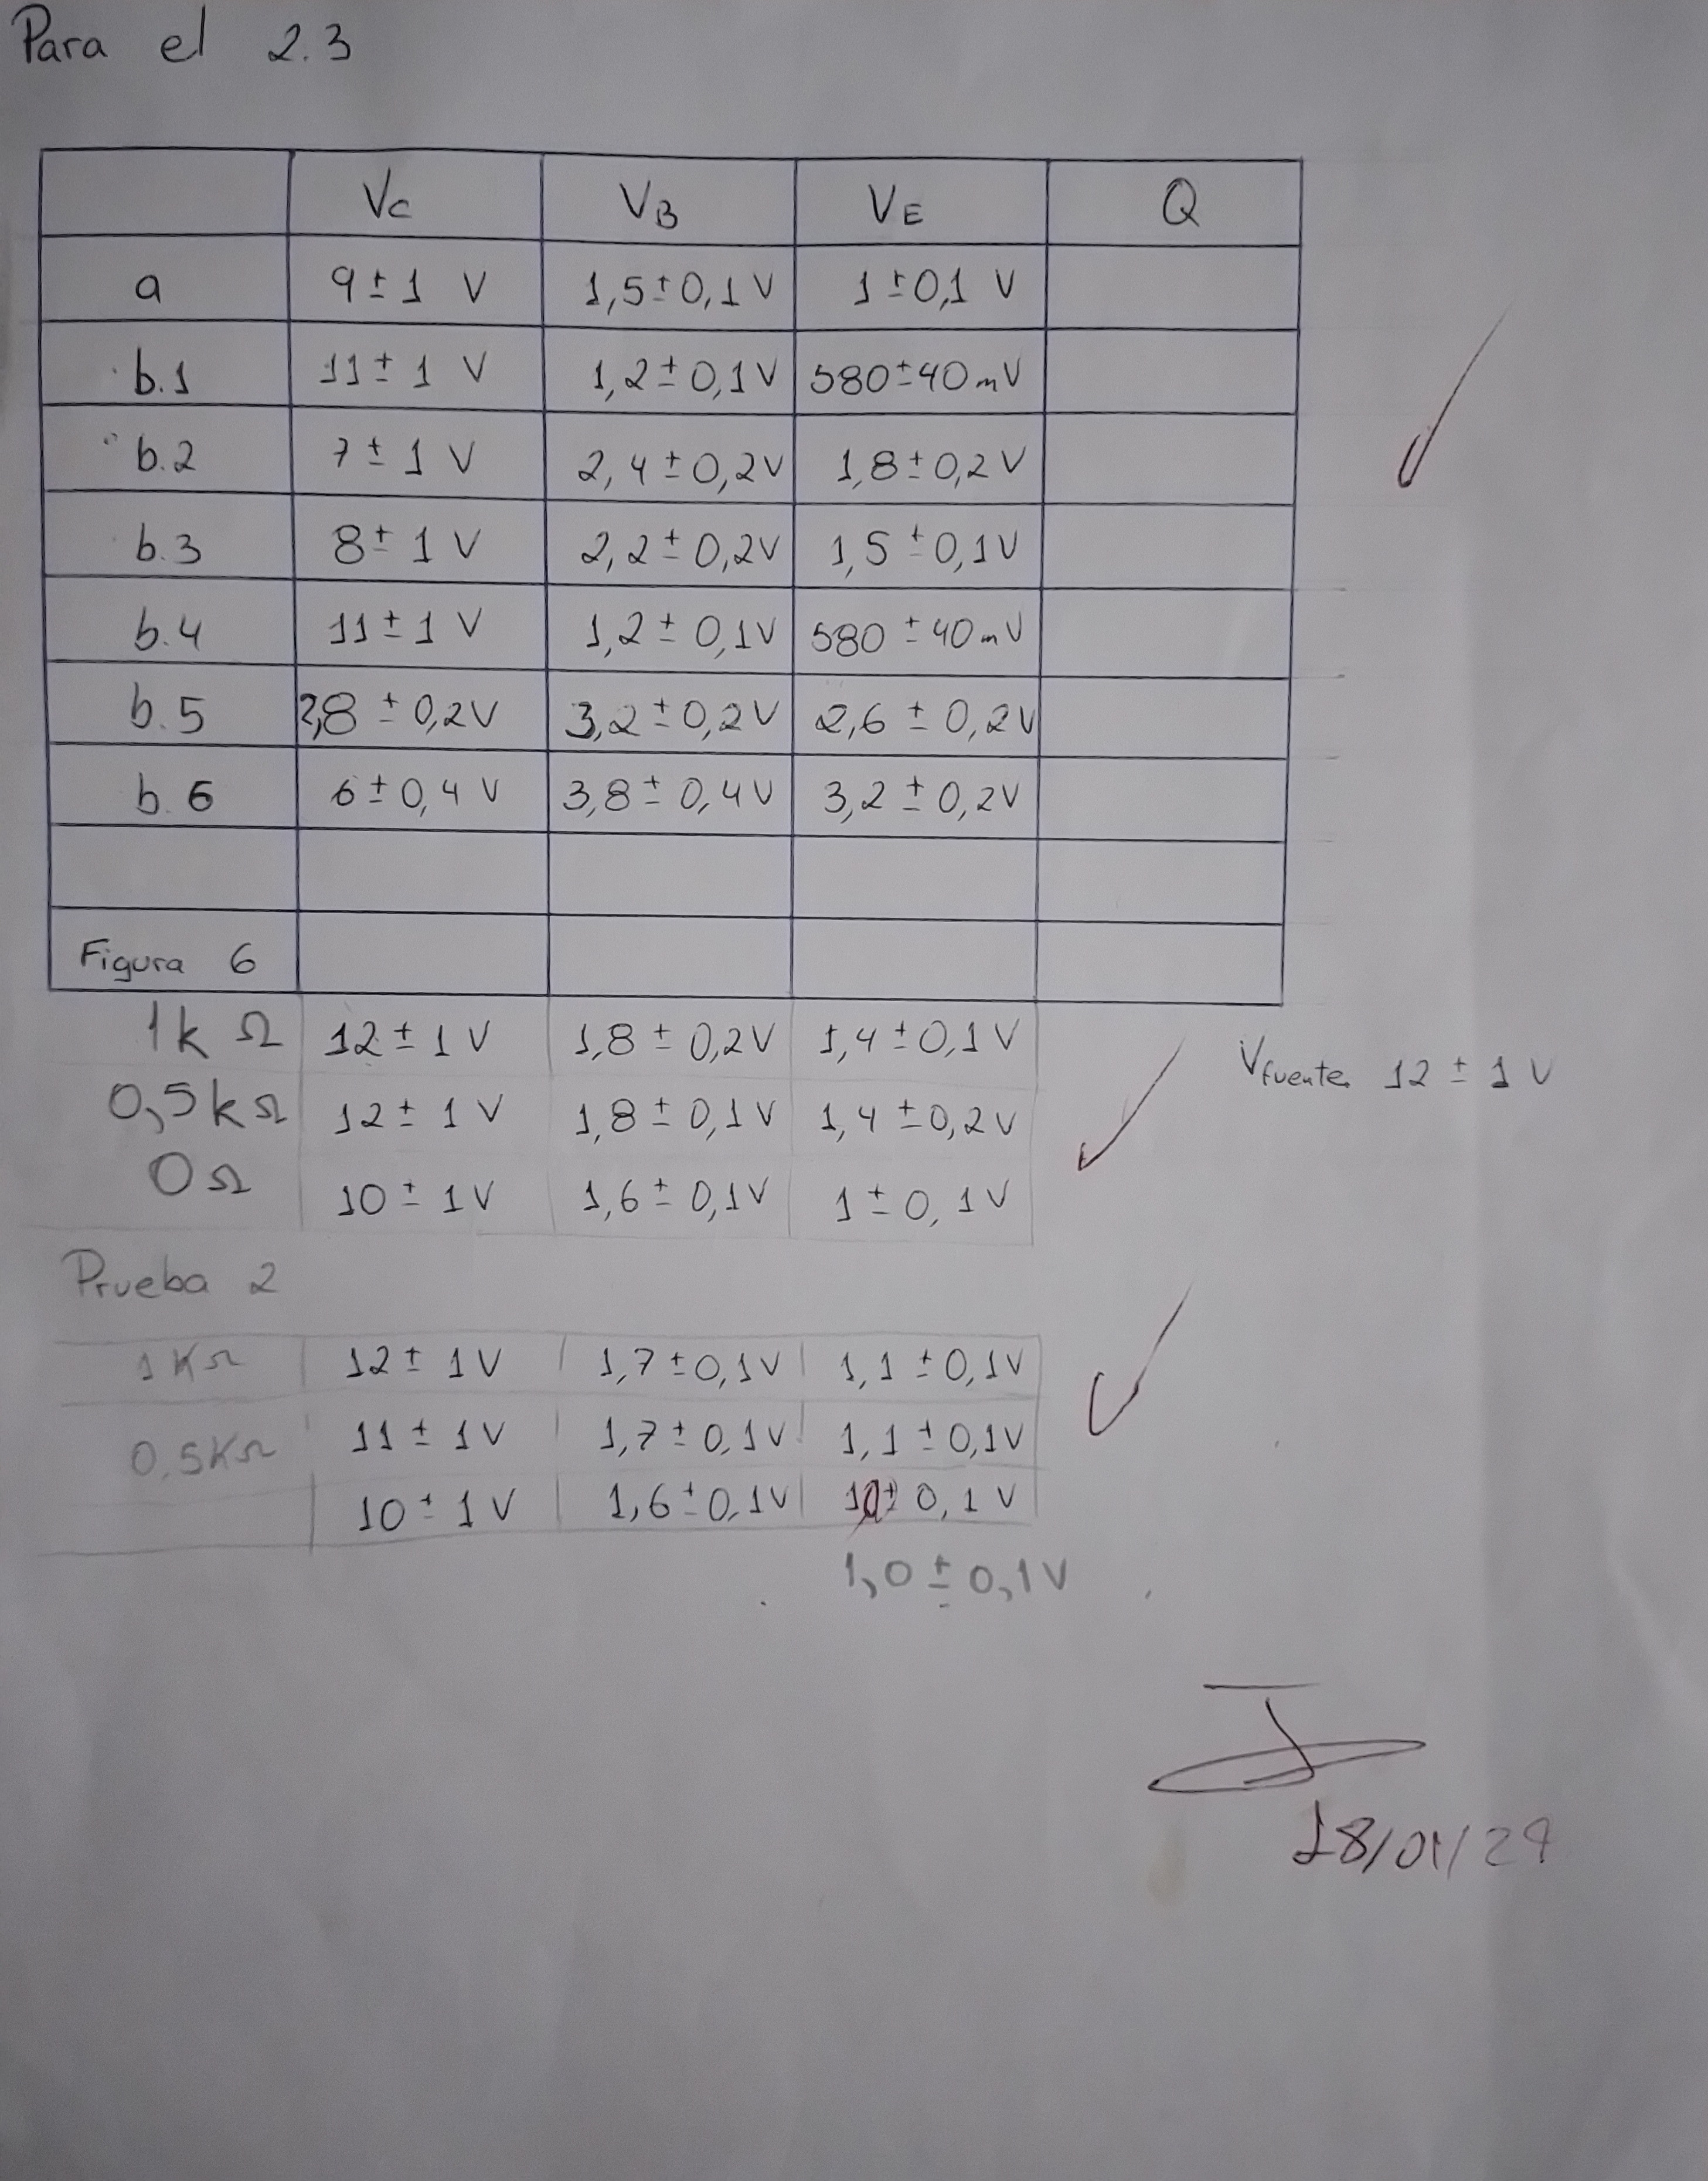
\includegraphics[height=10cm\textwidth]{hojadatos2.jpg}
        \caption{hoja de datos 2}
        \label{fig:hd2}
    \end{figure}

\end{document}